\begin{landscape}
\chapter{Projektmanagment}
Für die Organisation, der Aufgaben dieser Bachelorthesis, wurde ein Zeitplan aufgestellt. Um die Prozesse präzise zu steuern wurden ein Kanban-Board verwendet. Einige Task haben mehrere Kanban-Tickets erhalten, um ein iteratives Vorgehen zu ermöglichen.
\section{Zeitplan}
\begin{figure}[H]
  \centering
  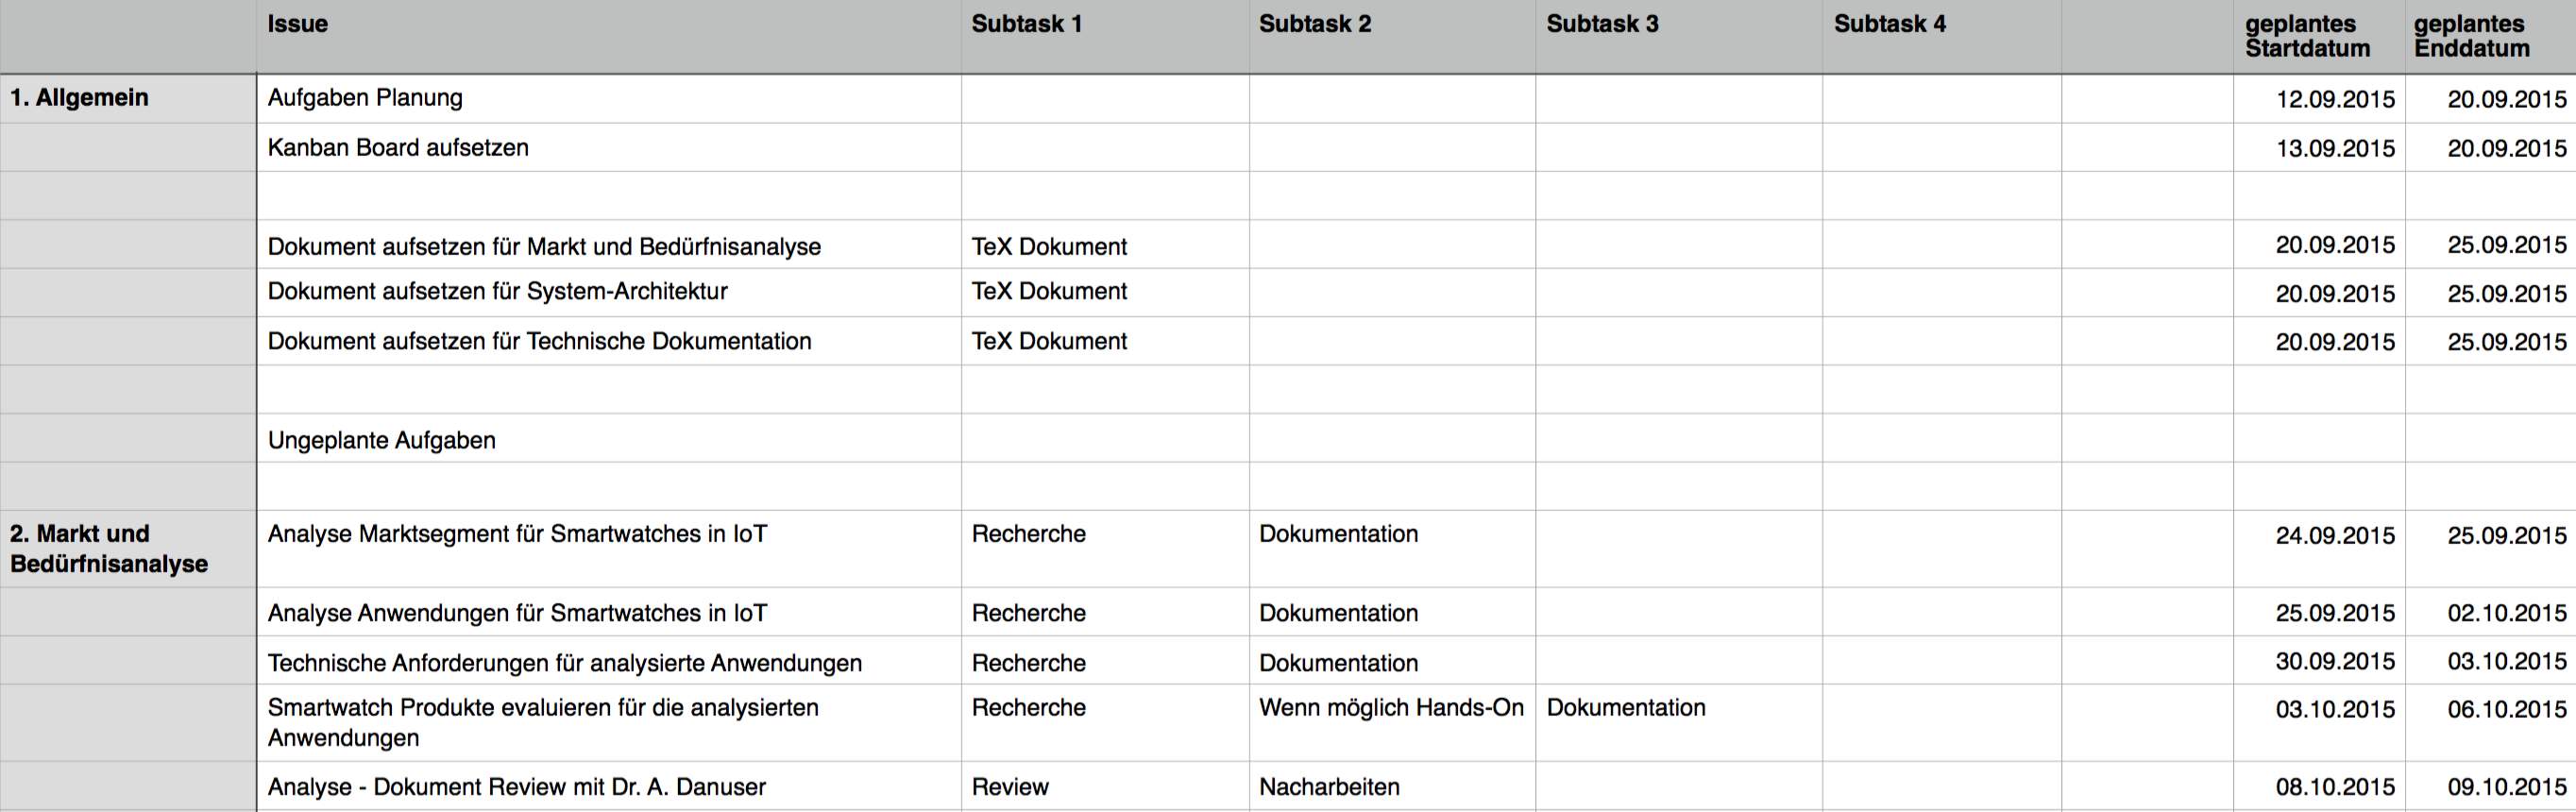
\includegraphics[scale=0.5]{98_Bilder/98_Anhang/zeitplanung_1}
  \caption[Zeitplan Teil 1]{Zeitplan der Bachelorthesis Teil 1}
\end{figure}
\begin{figure}[H]
  \centering
  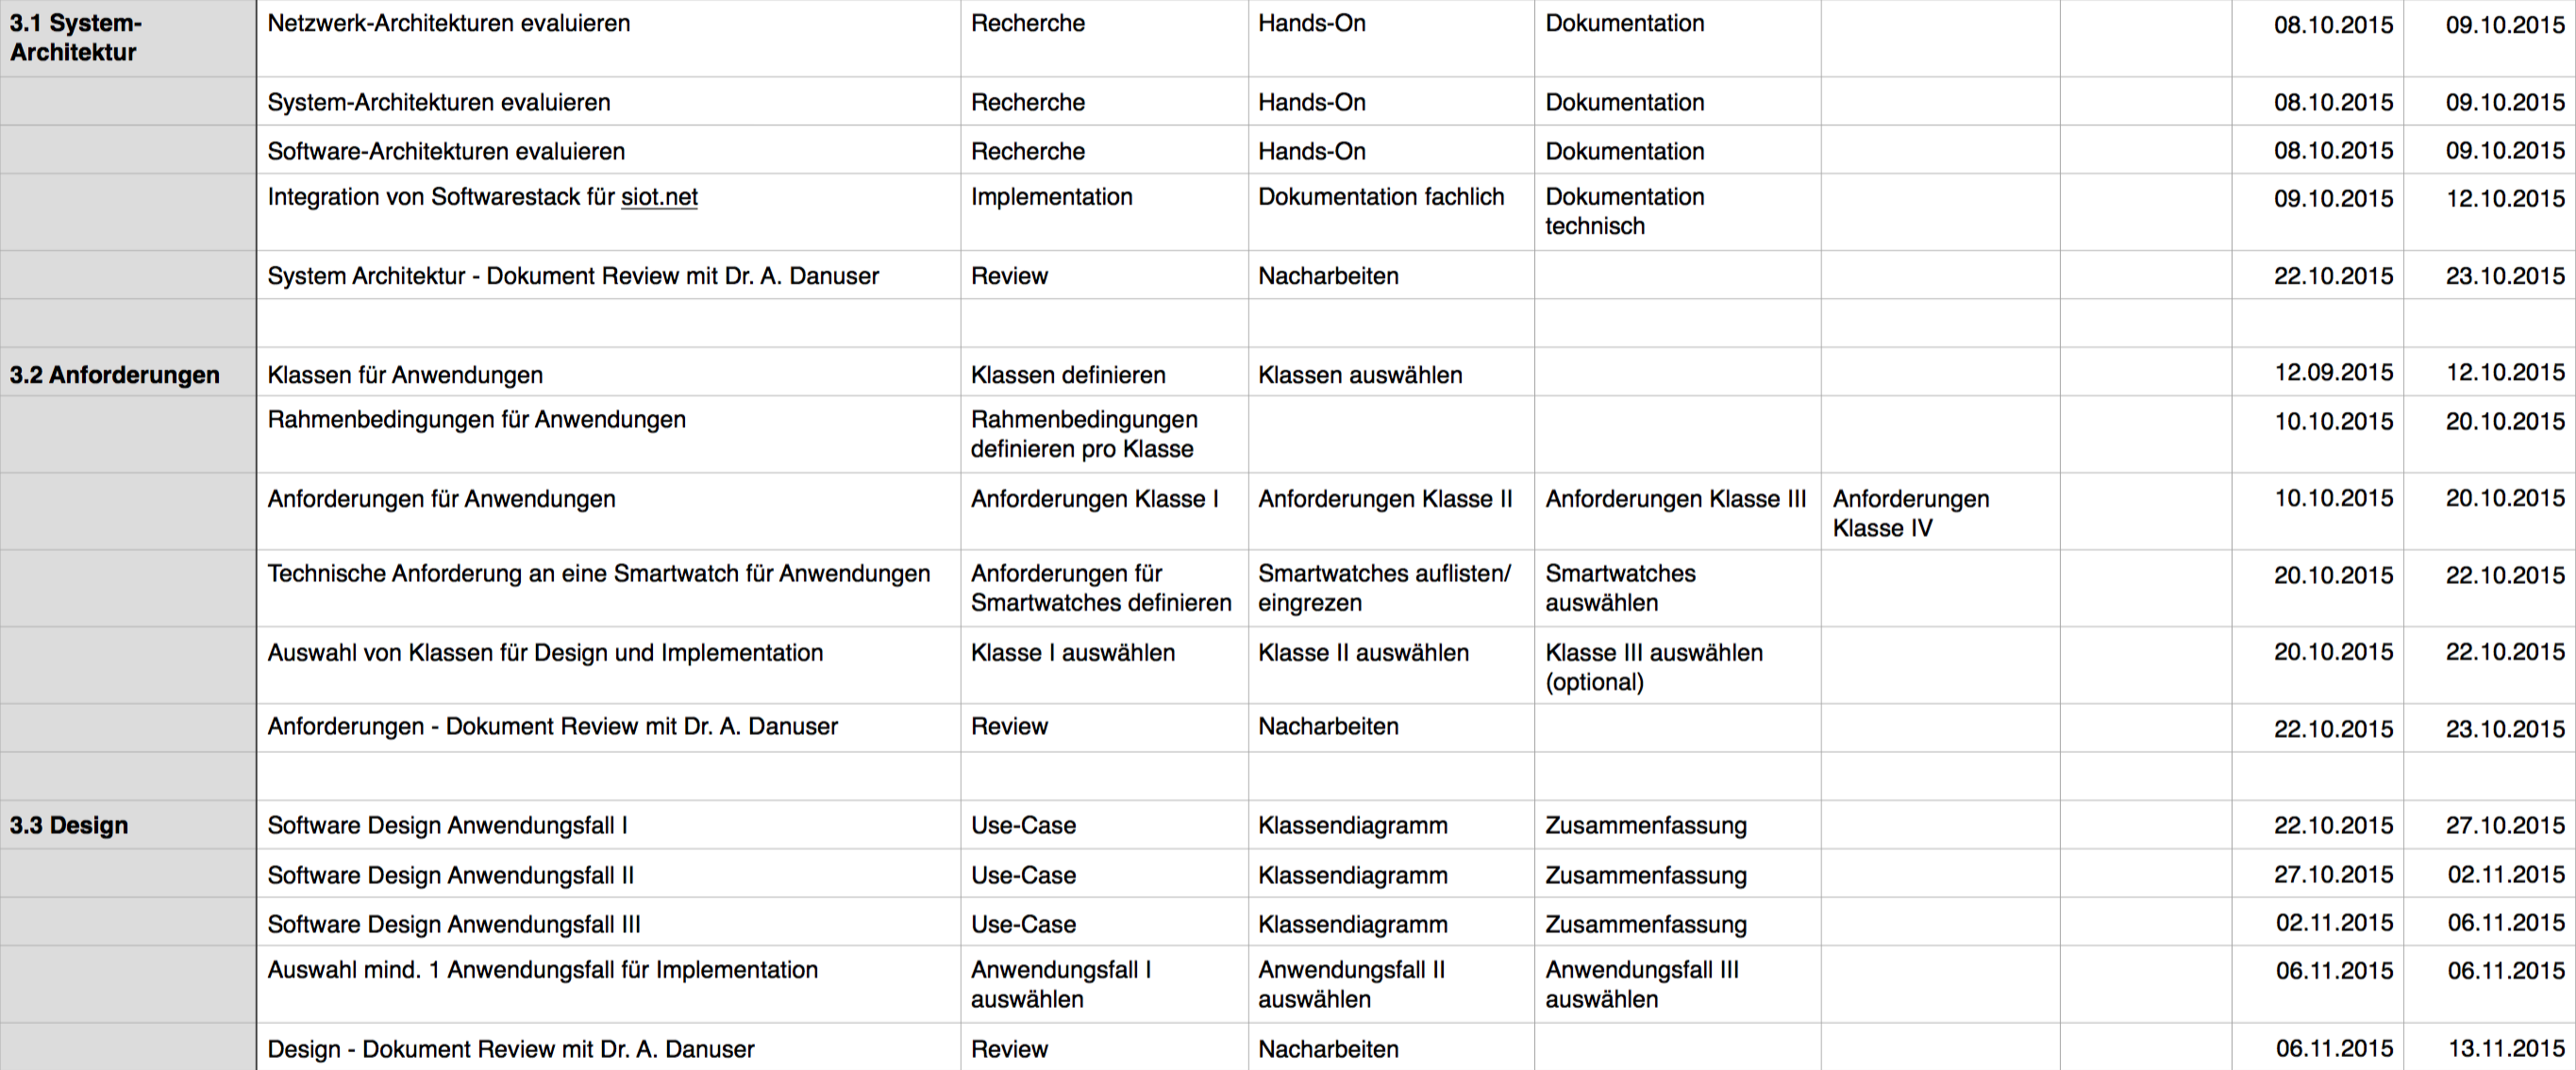
\includegraphics[scale=0.5]{98_Bilder/98_Anhang/zeitplanung_2}
  \caption[Zeitplan Teil 2]{Zeitplan der Bachelorthesis Teil 2}
\end{figure}
\begin{figure}[H]
  \centering
  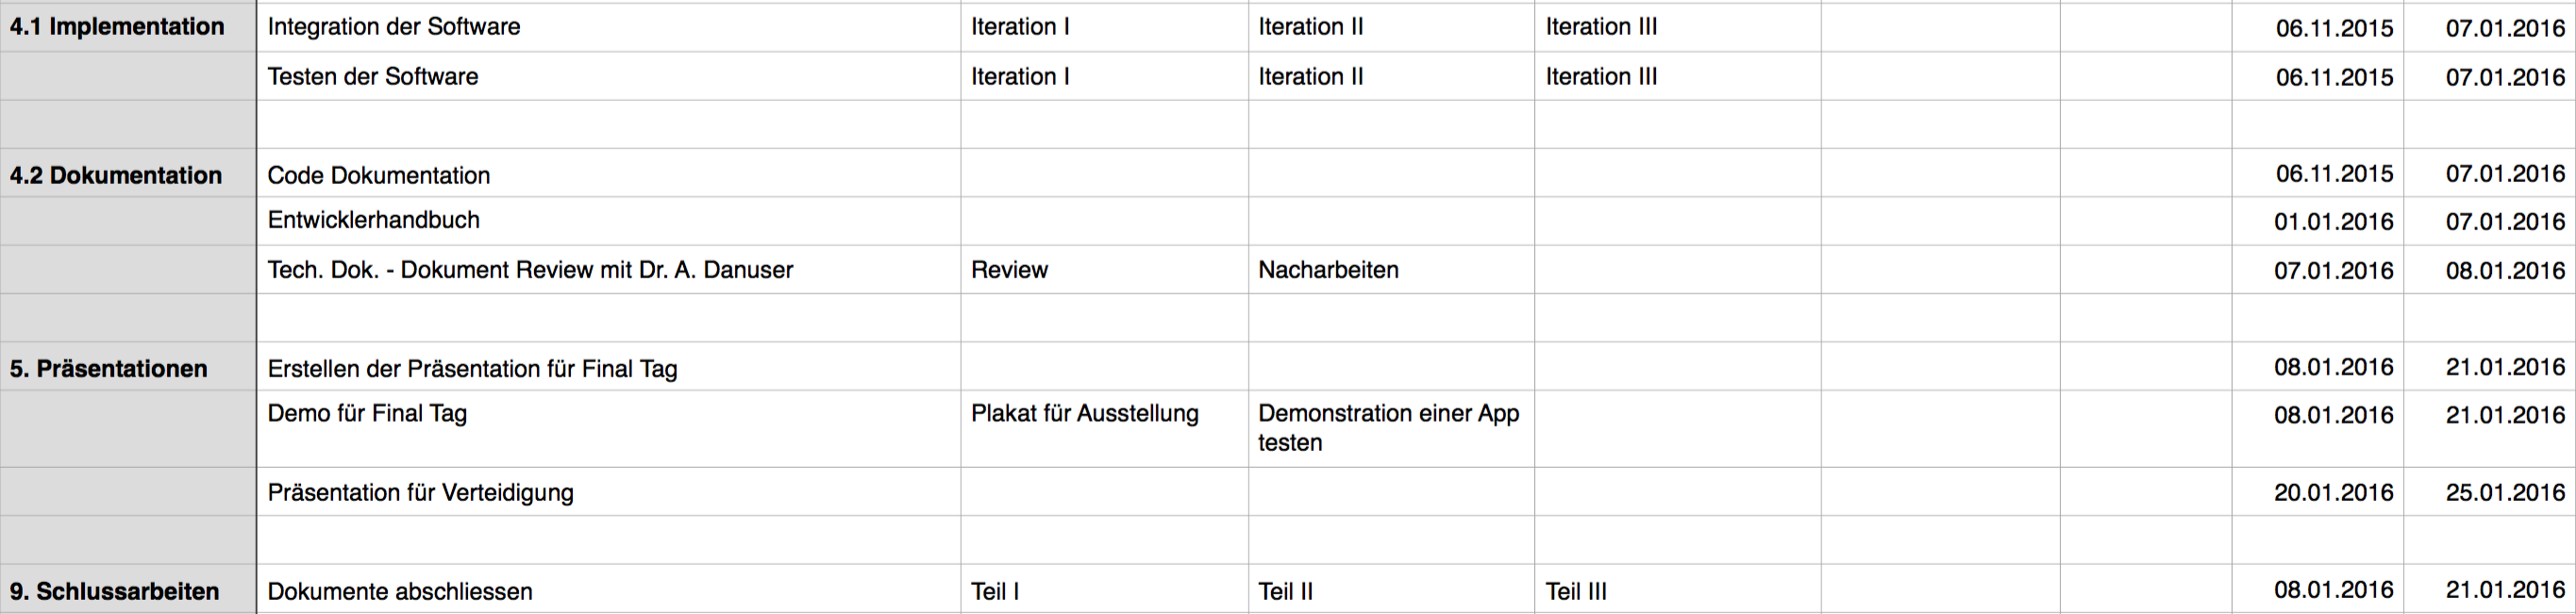
\includegraphics[scale=0.5]{98_Bilder/98_Anhang/zeitplanung_3}
  \caption[Zeitplan Teil 3]{Zeitplan der Bachelorthesis Teil 3}
\end{figure}
\end{landscape}
\begin{landscape}
\section{Kanban-Board Verlauf}
In diesem Abschnitt ist der Verlauf der Kanban-Tickets ersichtlich.
\begin{figure}[H]
  \centering
  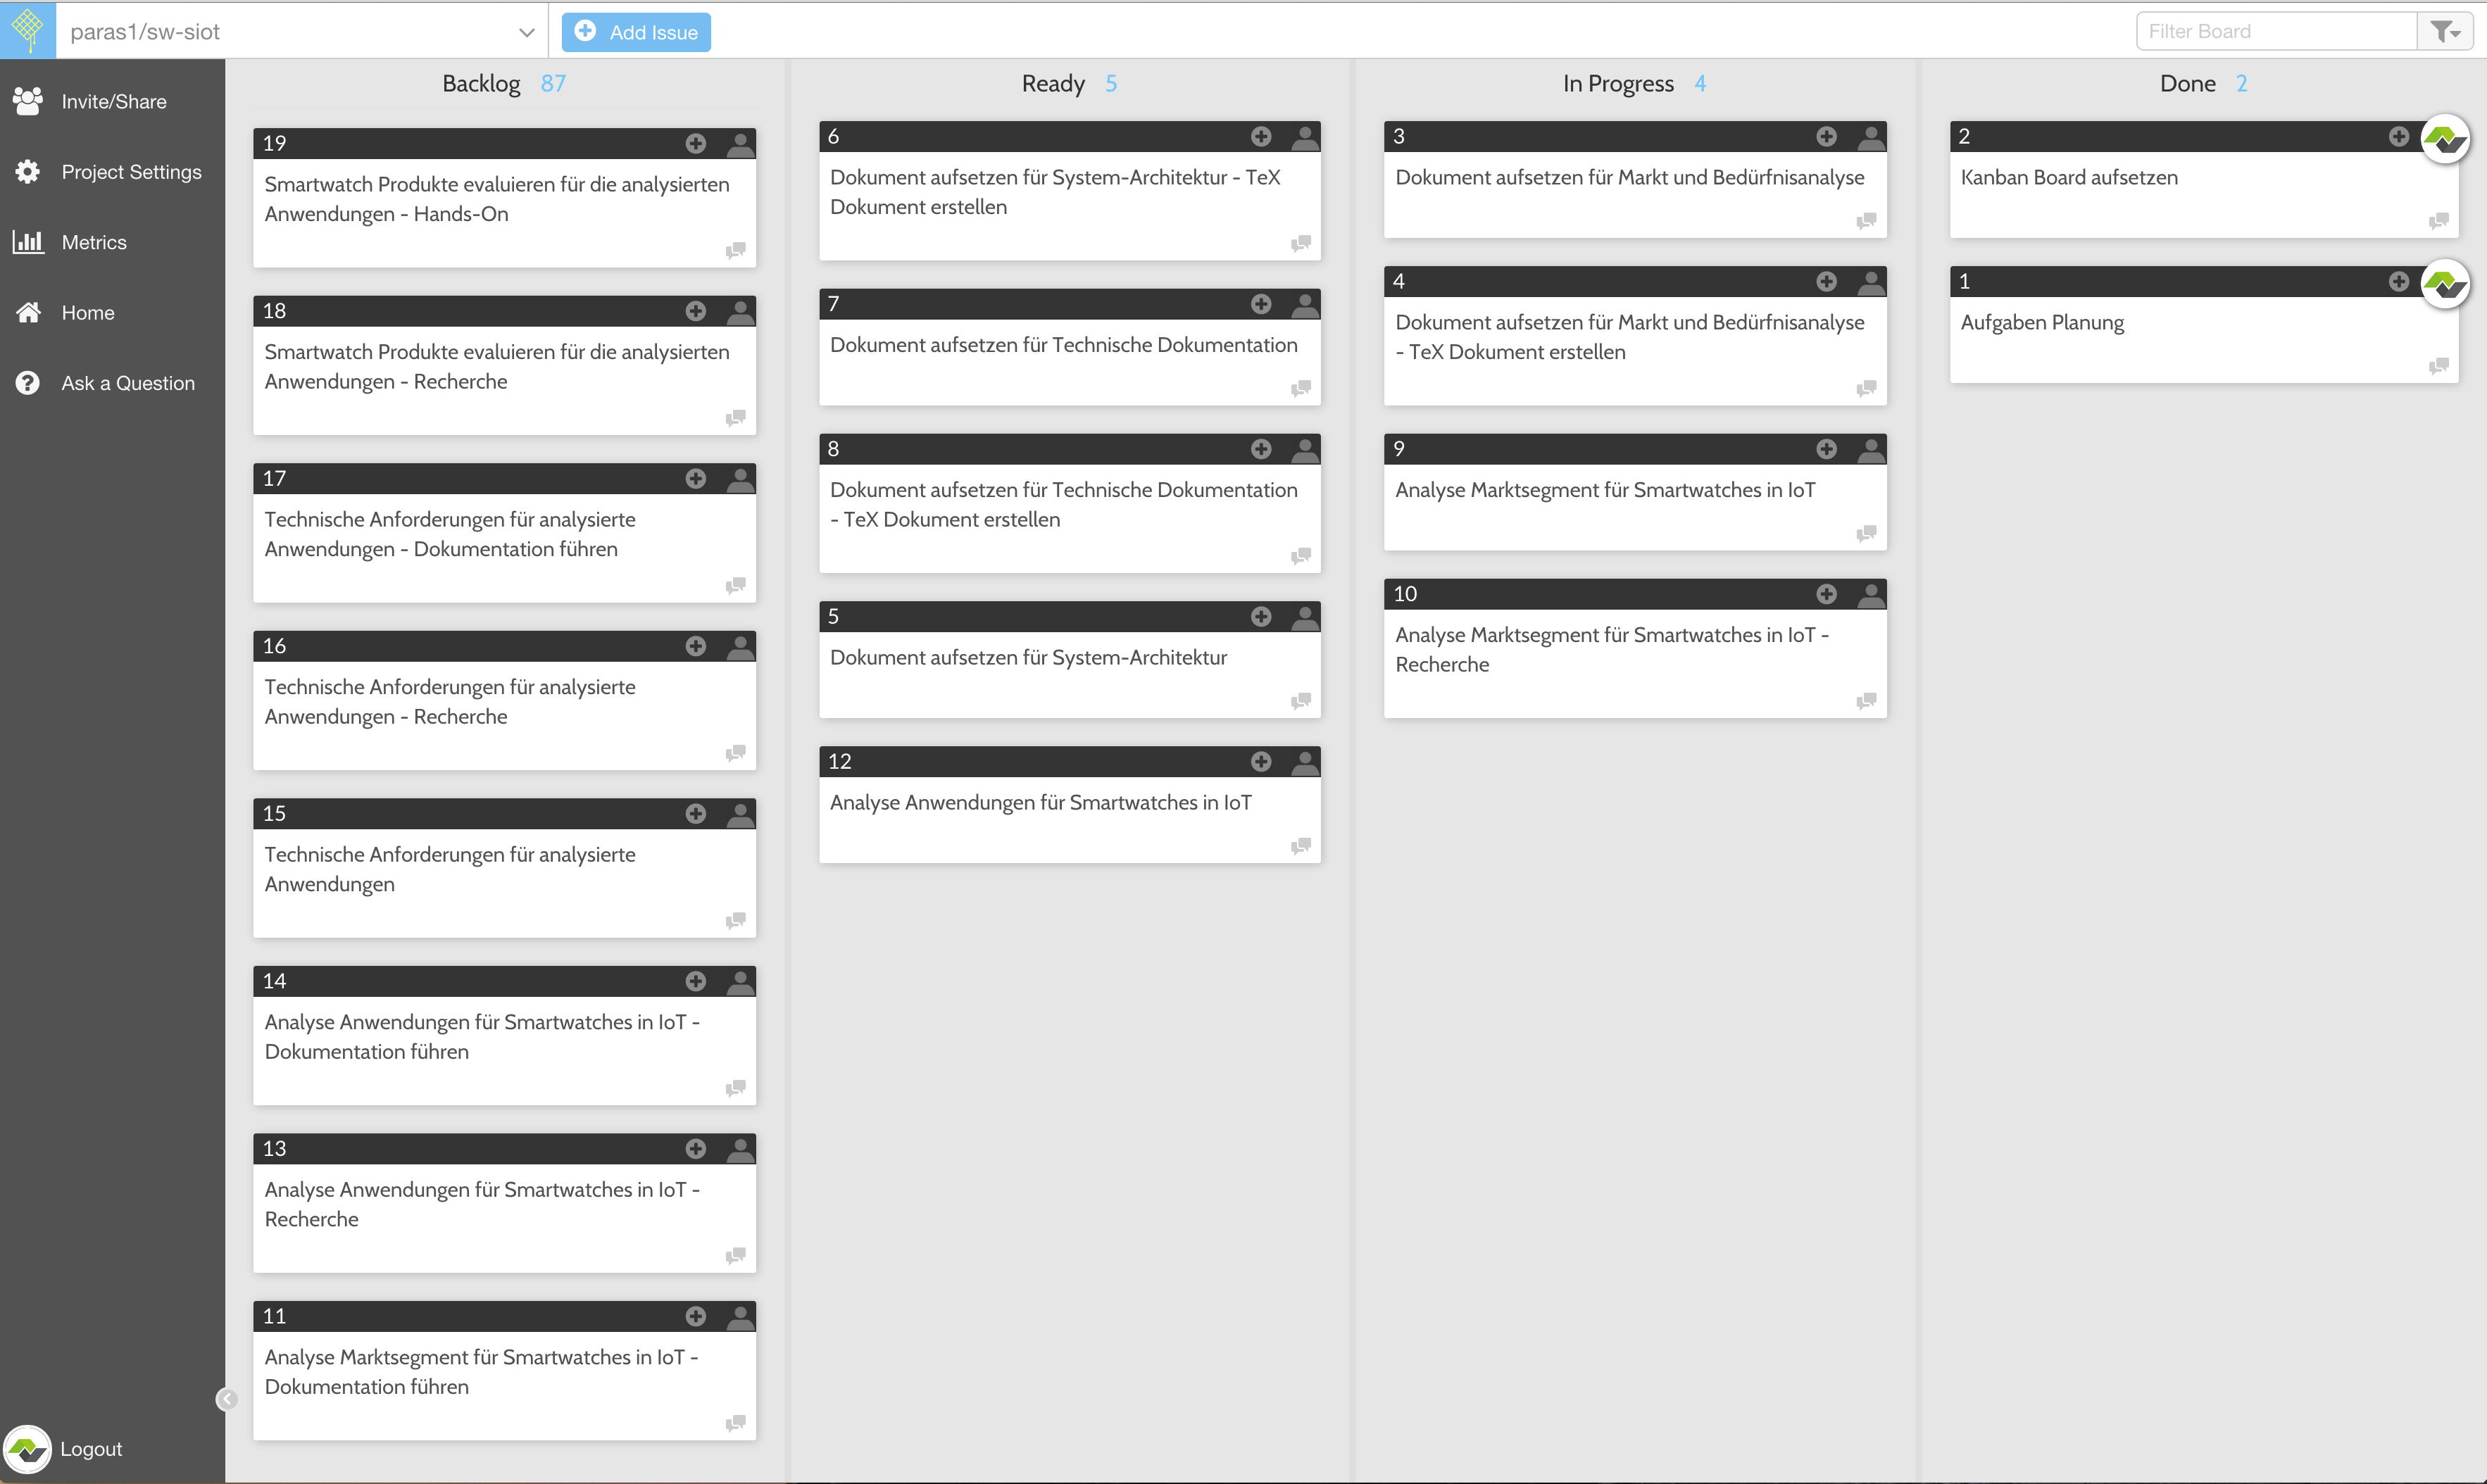
\includegraphics[scale=0.37]{98_Bilder/98_Anhang/20150924_Kanban_board}
  \caption[Kanban-Board 24.09.2015]{Kanban-Board Fortschritt am 24.09.2015}
\end{figure}
\begin{figure}[H]
  \centering
  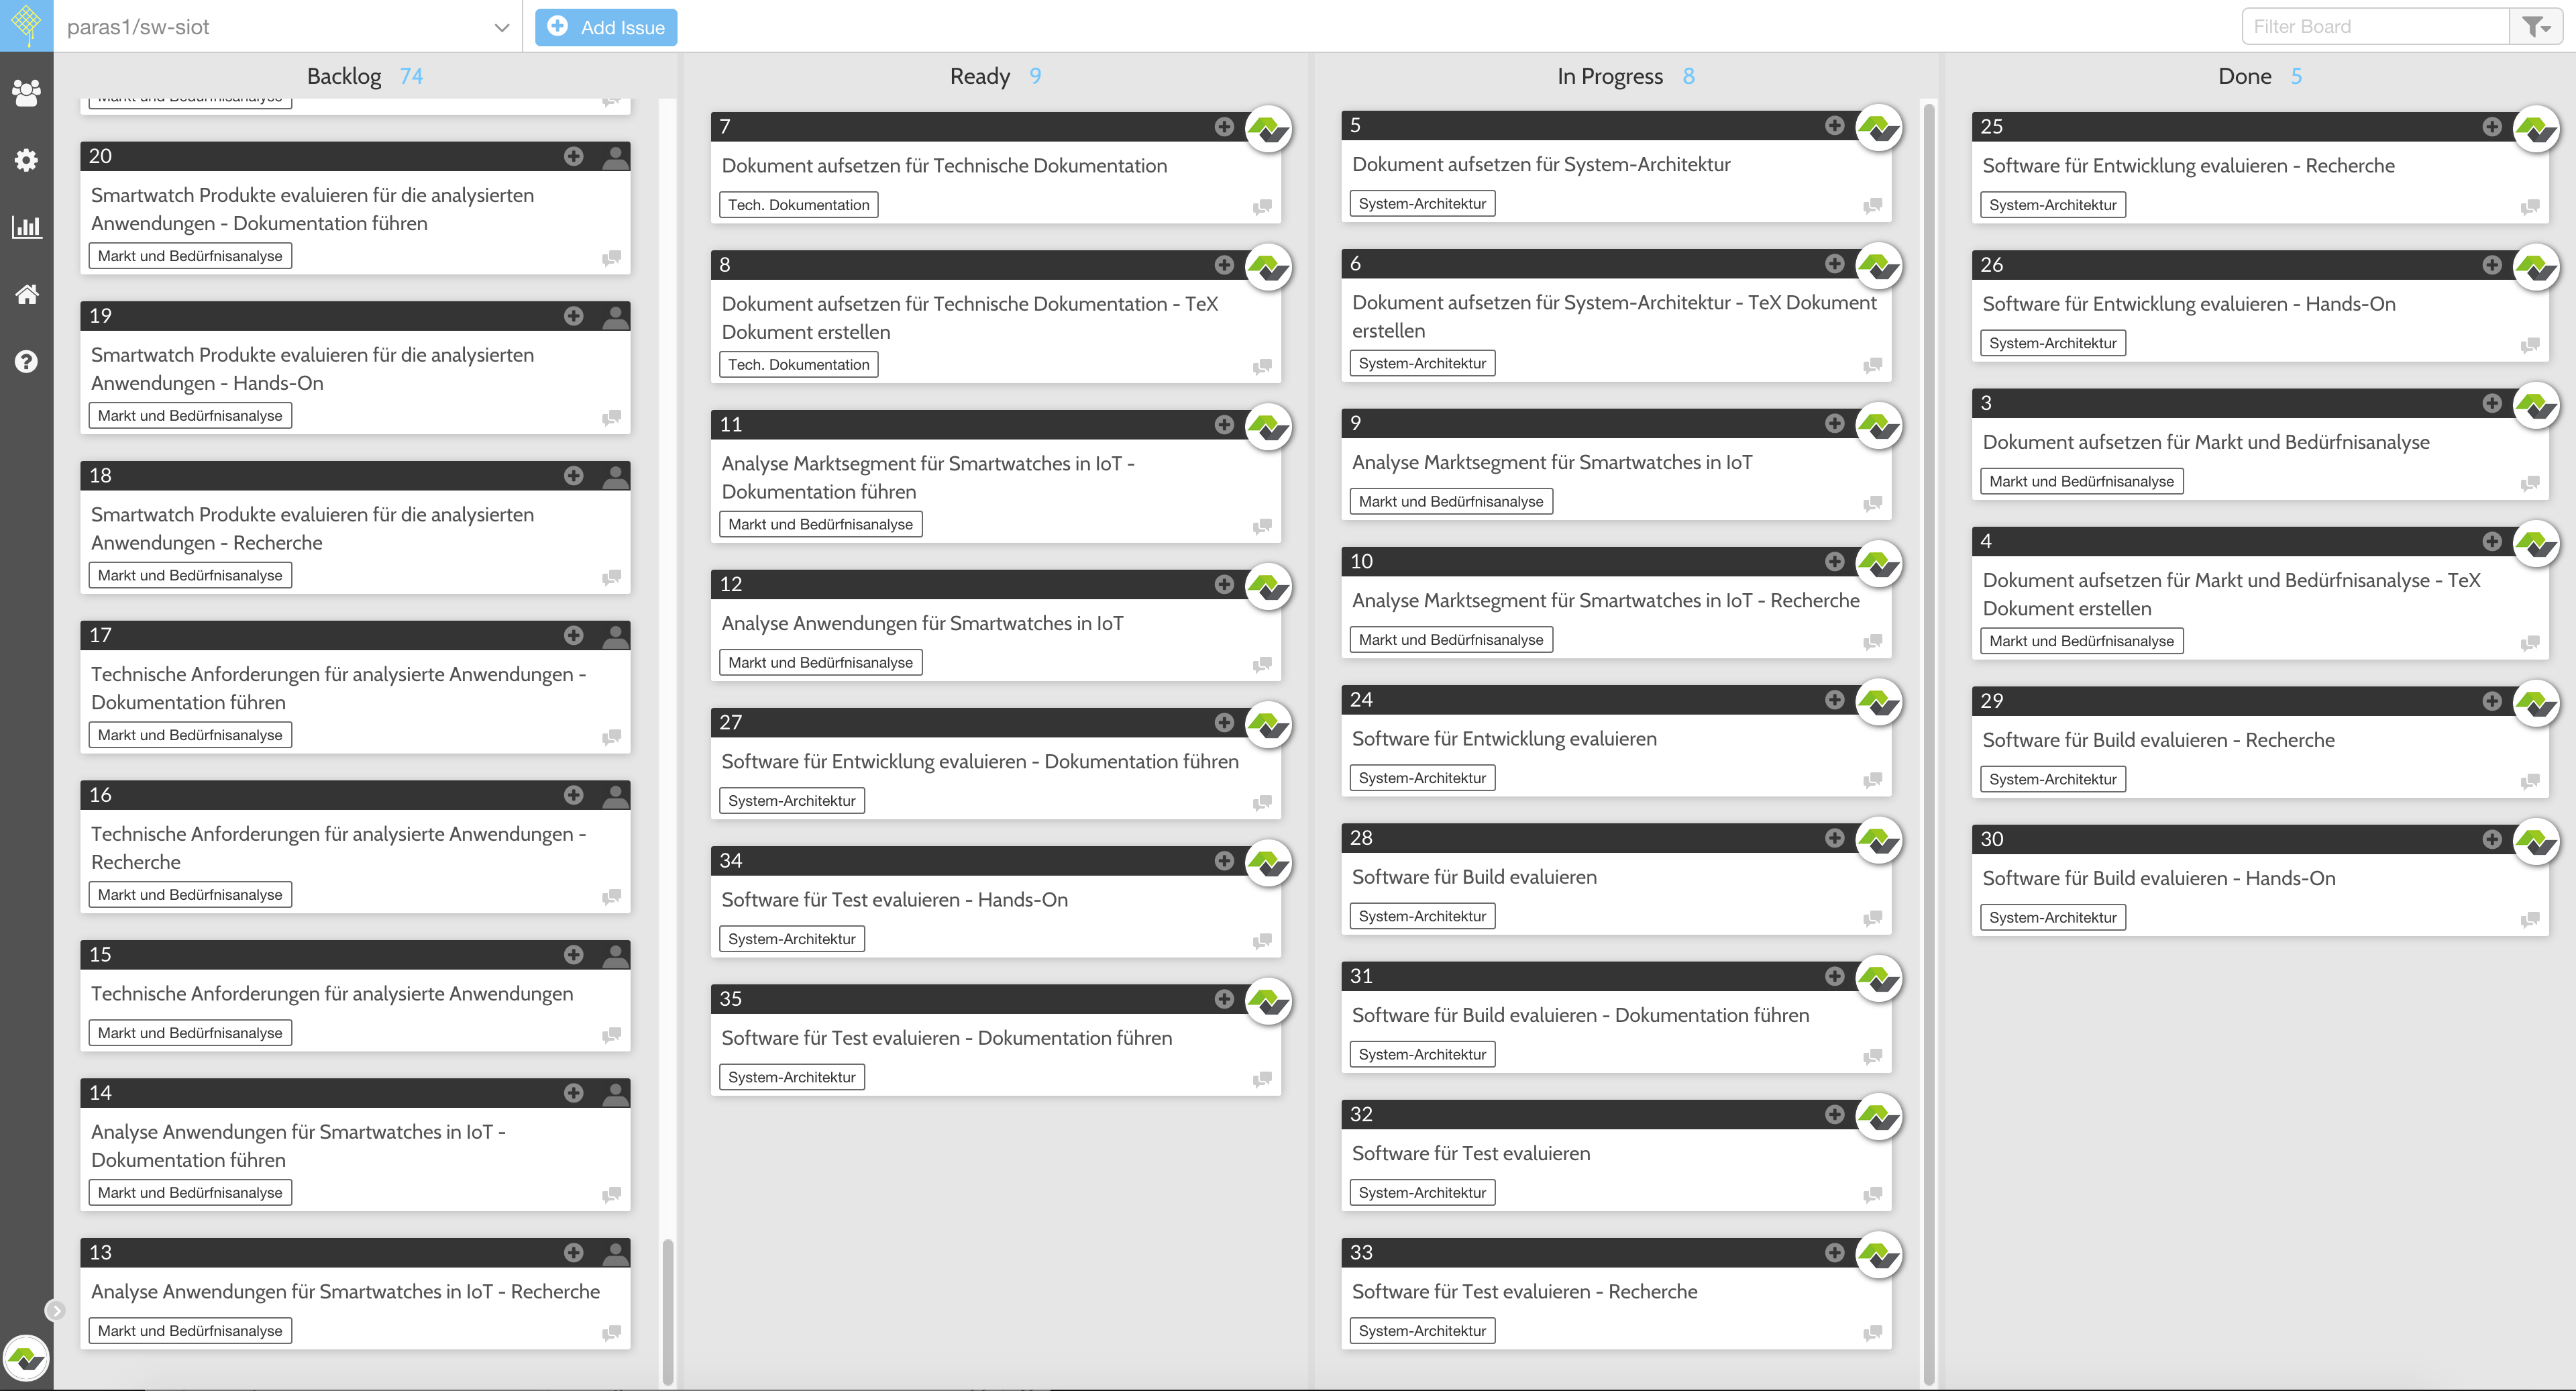
\includegraphics[scale=0.37]{98_Bilder/98_Anhang/20151009_Kanban_board}
  \caption[Kanban-Board 09.10.2015]{Kanban-Board Fortschritt am 09.10.2015}
\end{figure}
\begin{figure}[H]
  \centering
  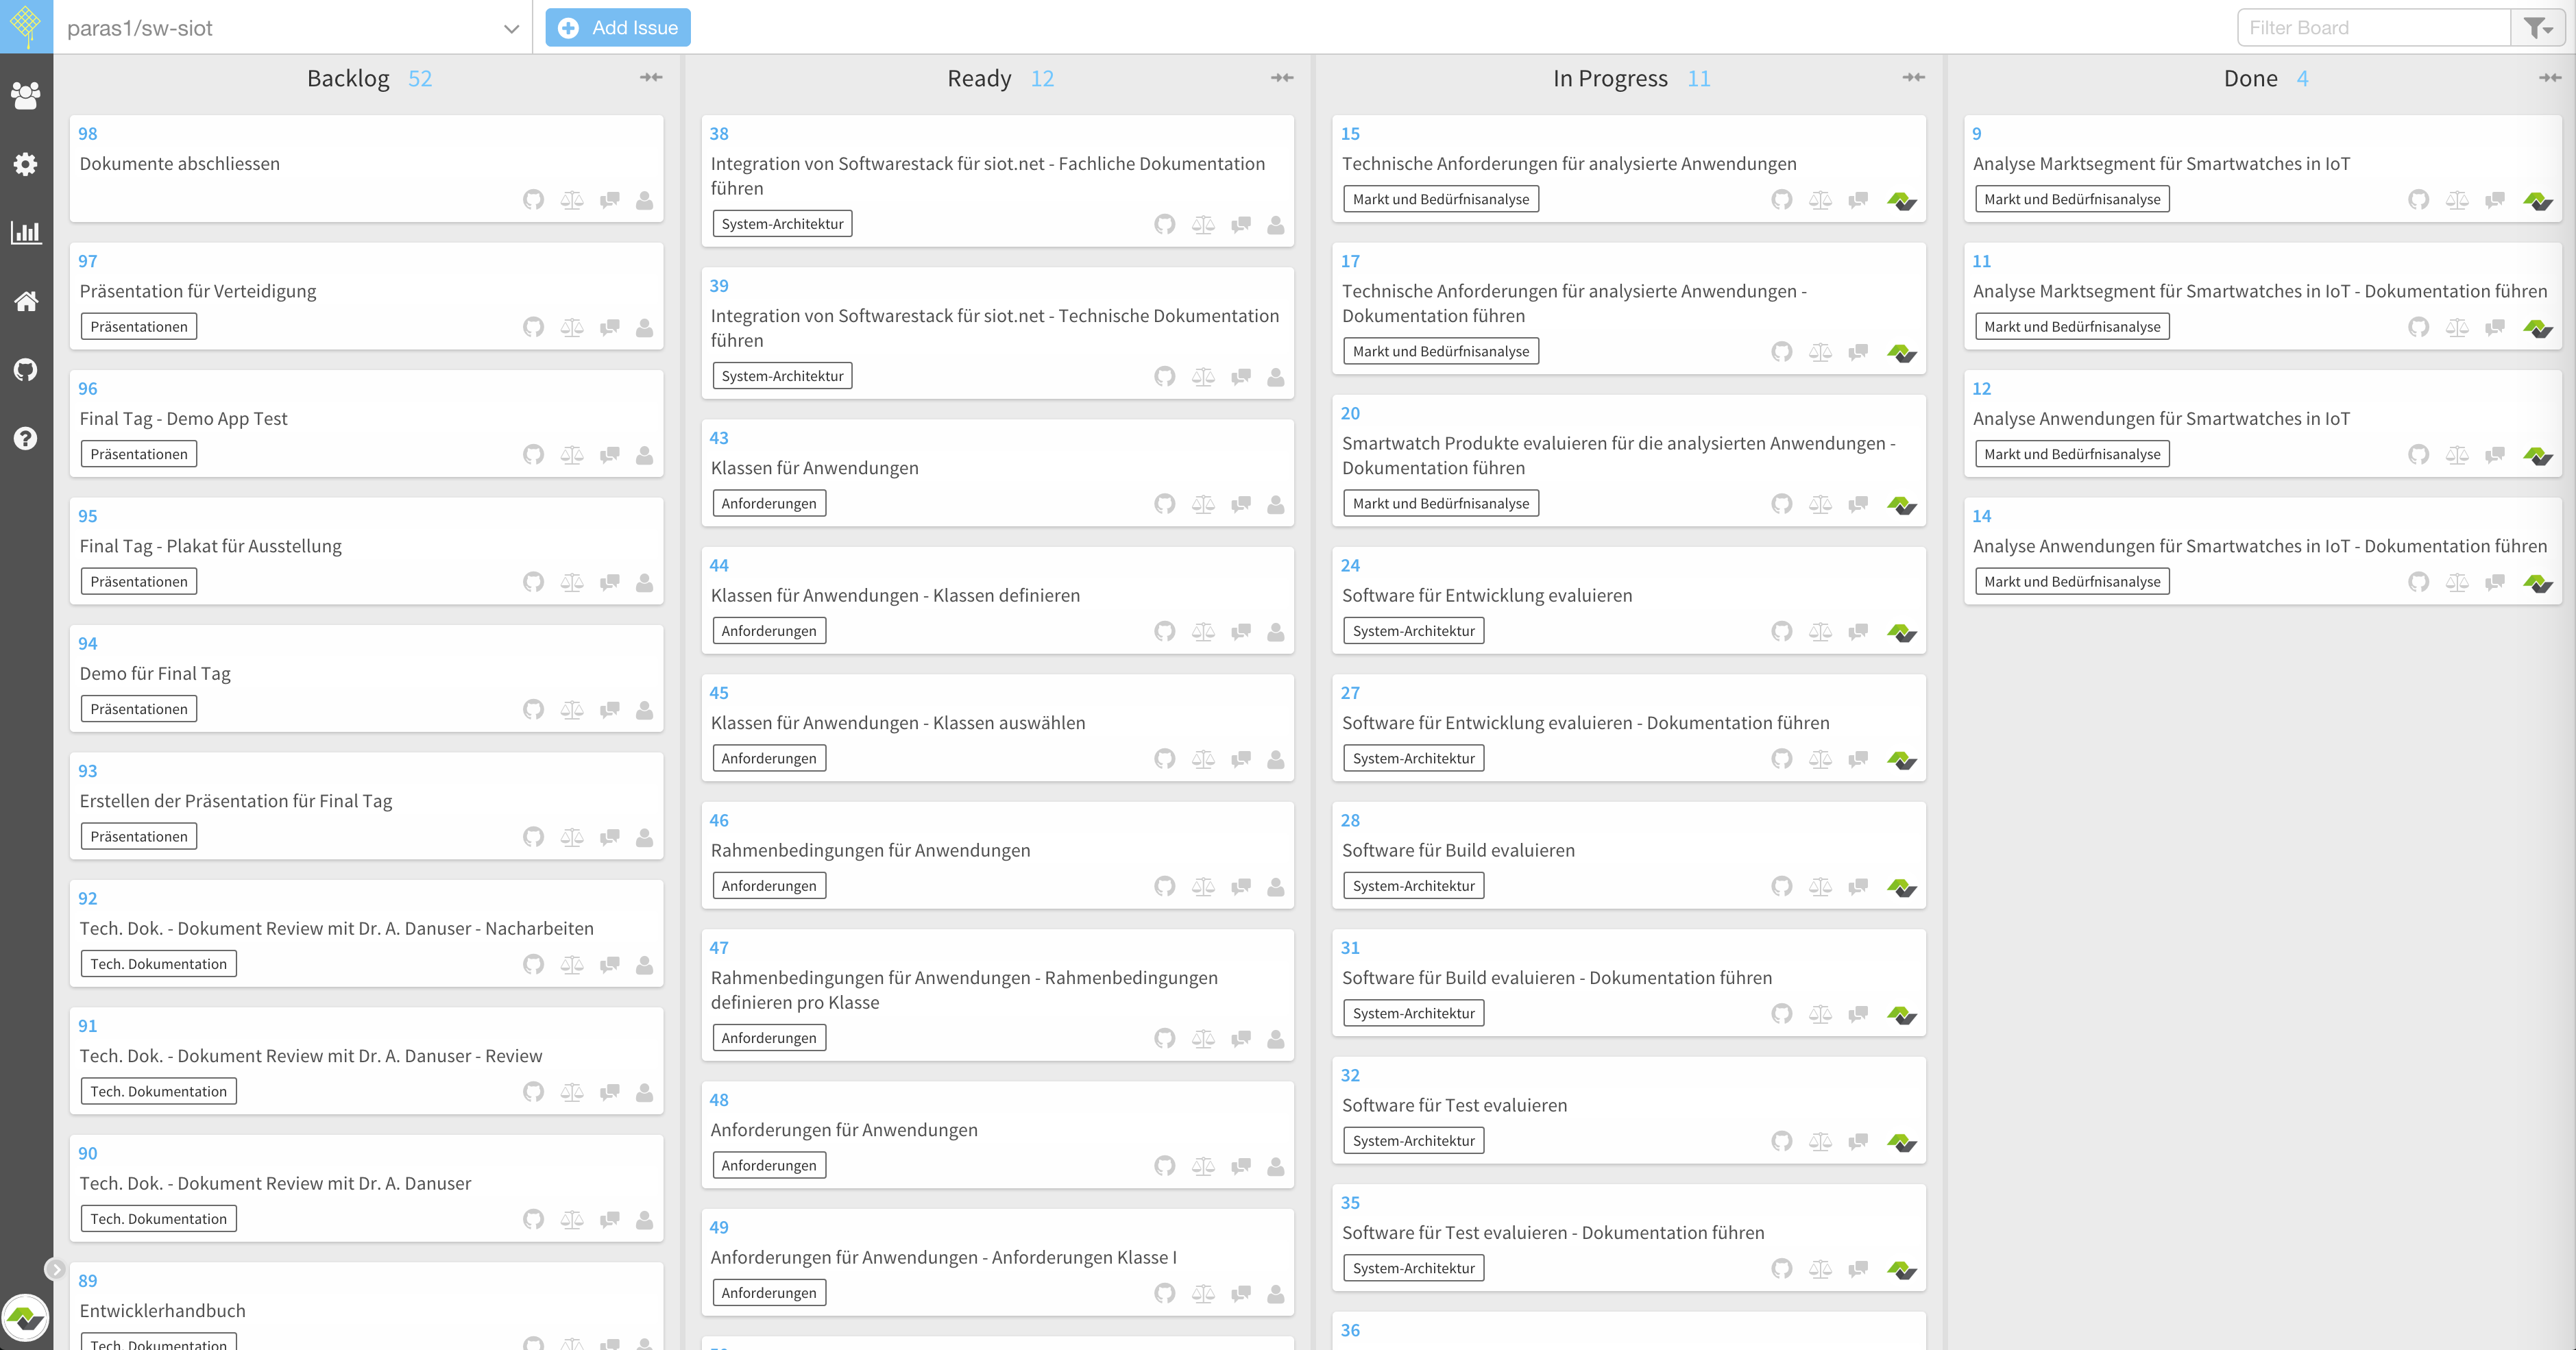
\includegraphics[scale=0.37]{98_Bilder/98_Anhang/20151130_Kanban_board}
  \caption[Kanban-Board 08.11.2015]{Kanban-Board Fortschritt am 08.11.2015}
\end{figure}
\begin{figure}[H]
  \centering
  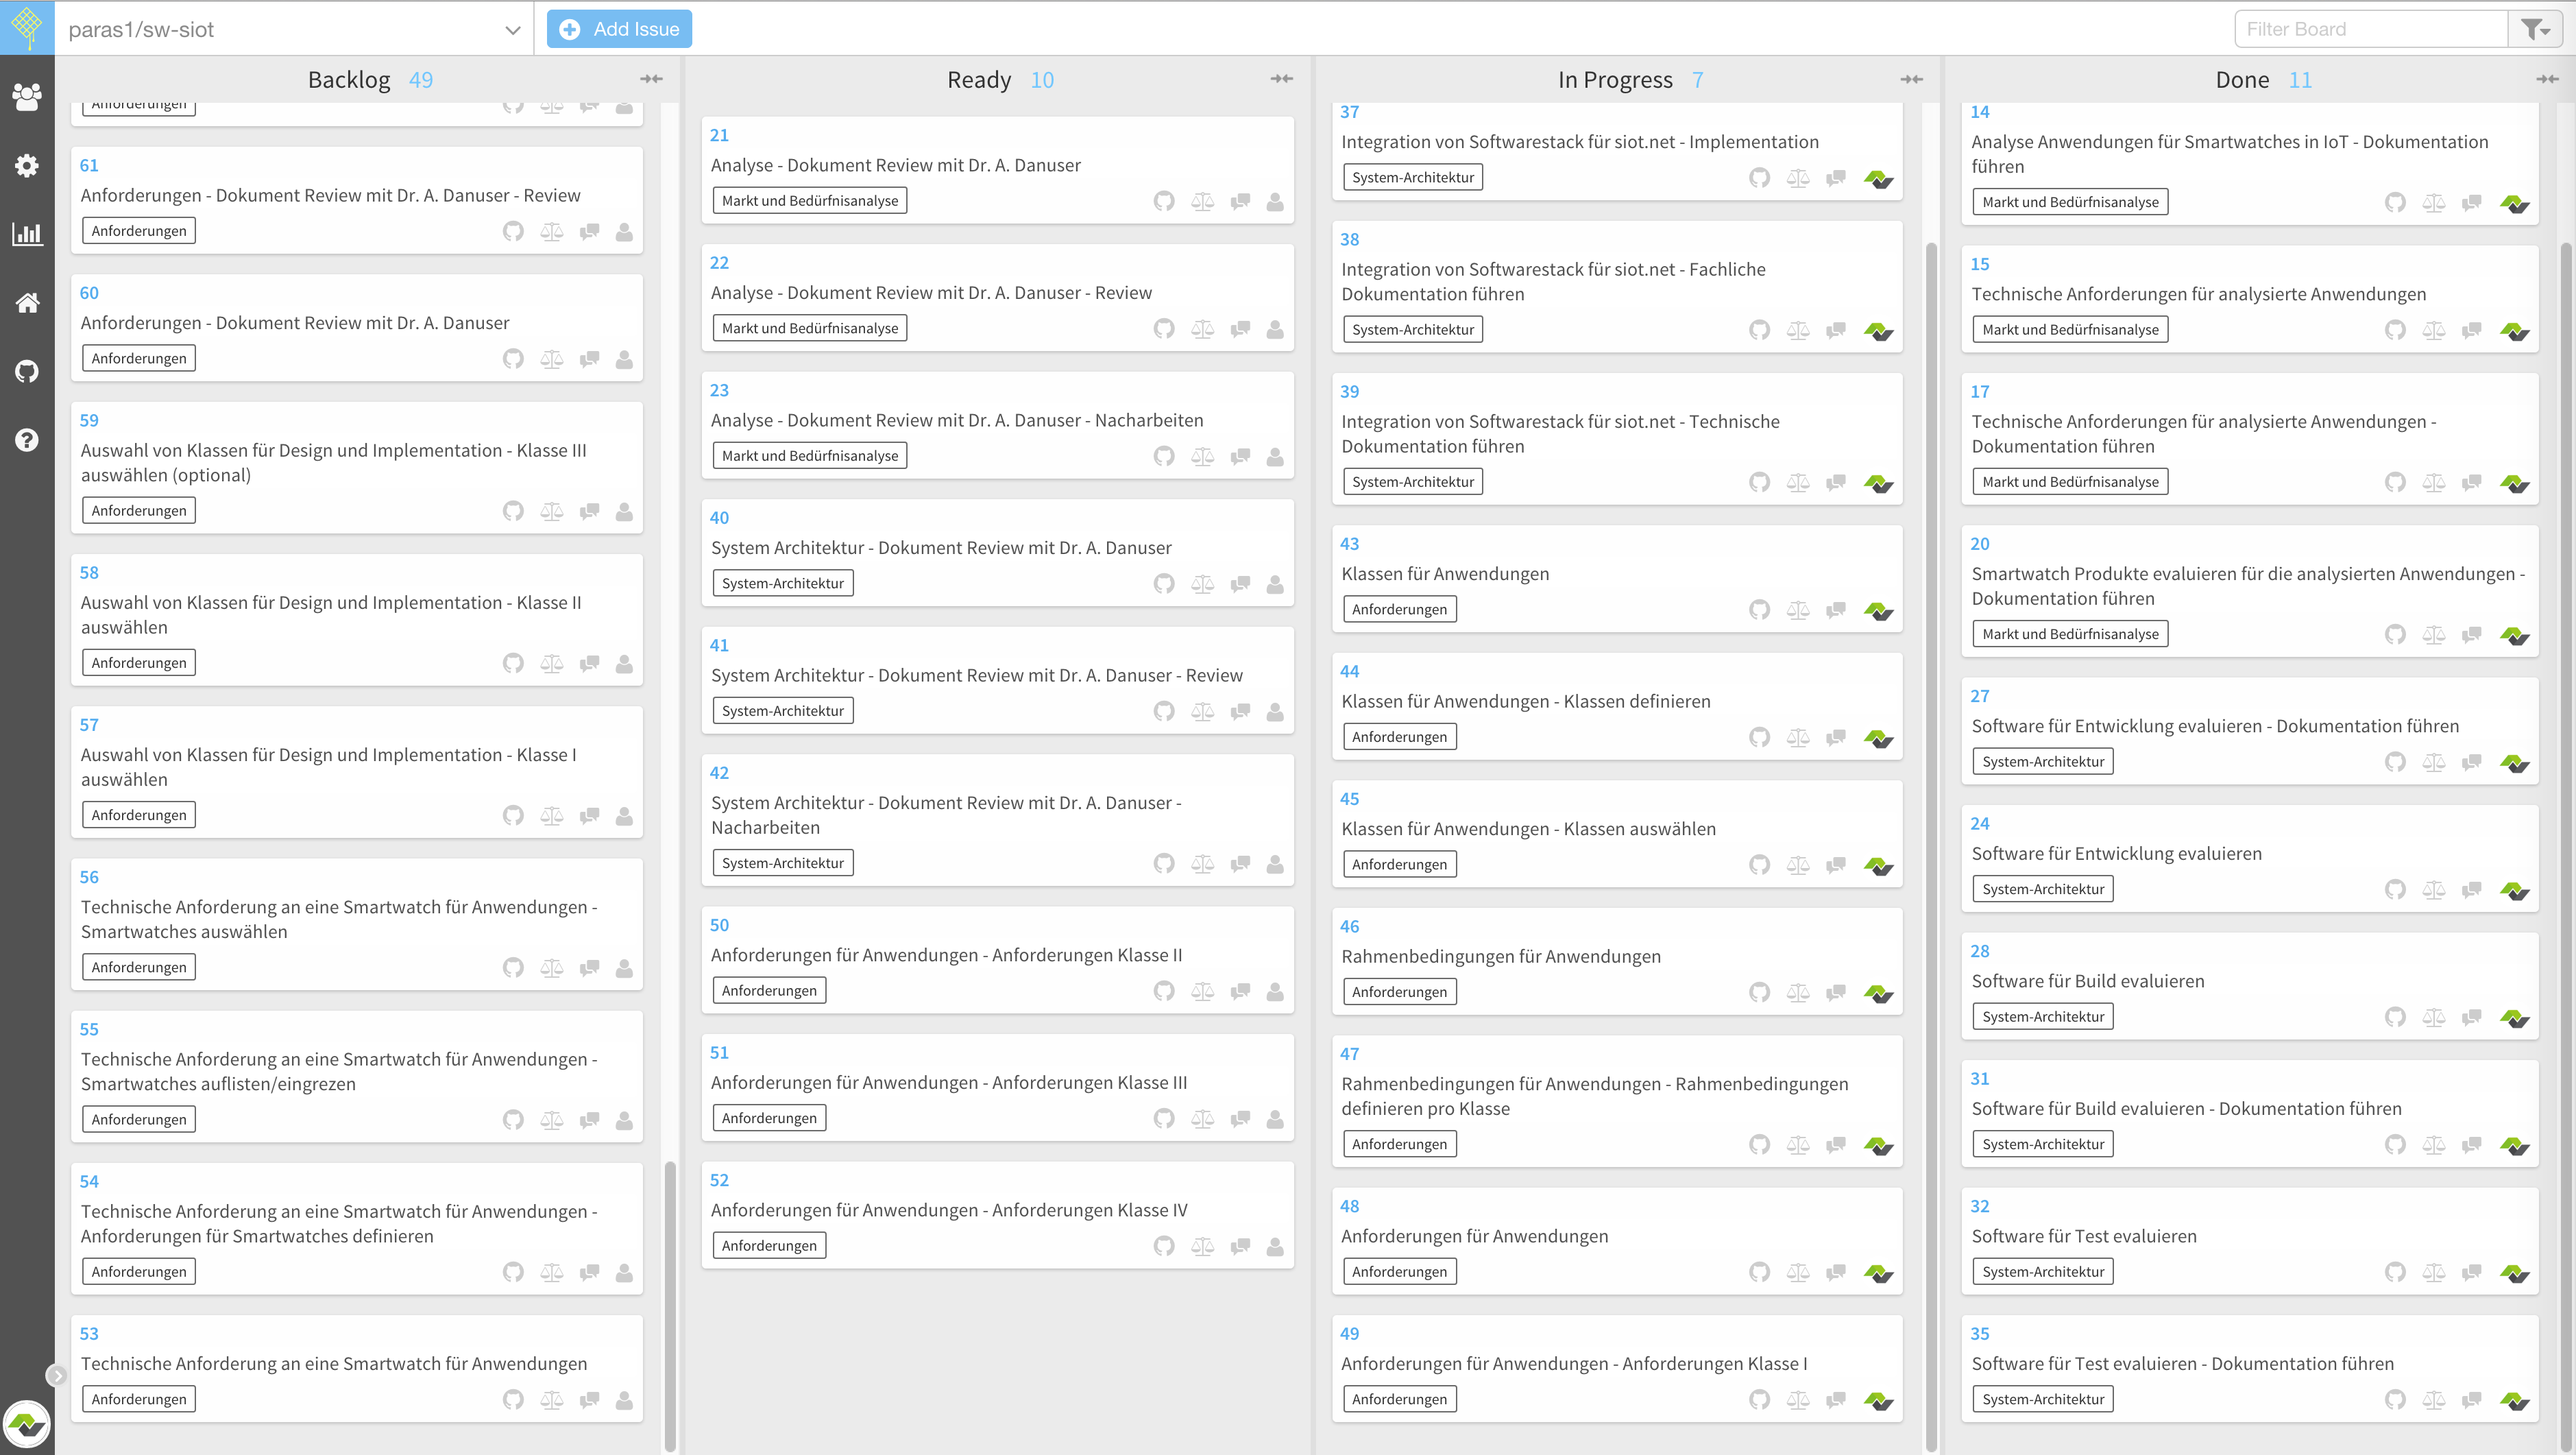
\includegraphics[scale=0.37]{98_Bilder/98_Anhang/20151204_Kanban_board}
  \caption[Kanban-Board 04.12.2015]{Kanban-Board Fortschritt am 04.12.2015}
\end{figure}
\begin{figure}[H]
  \centering
  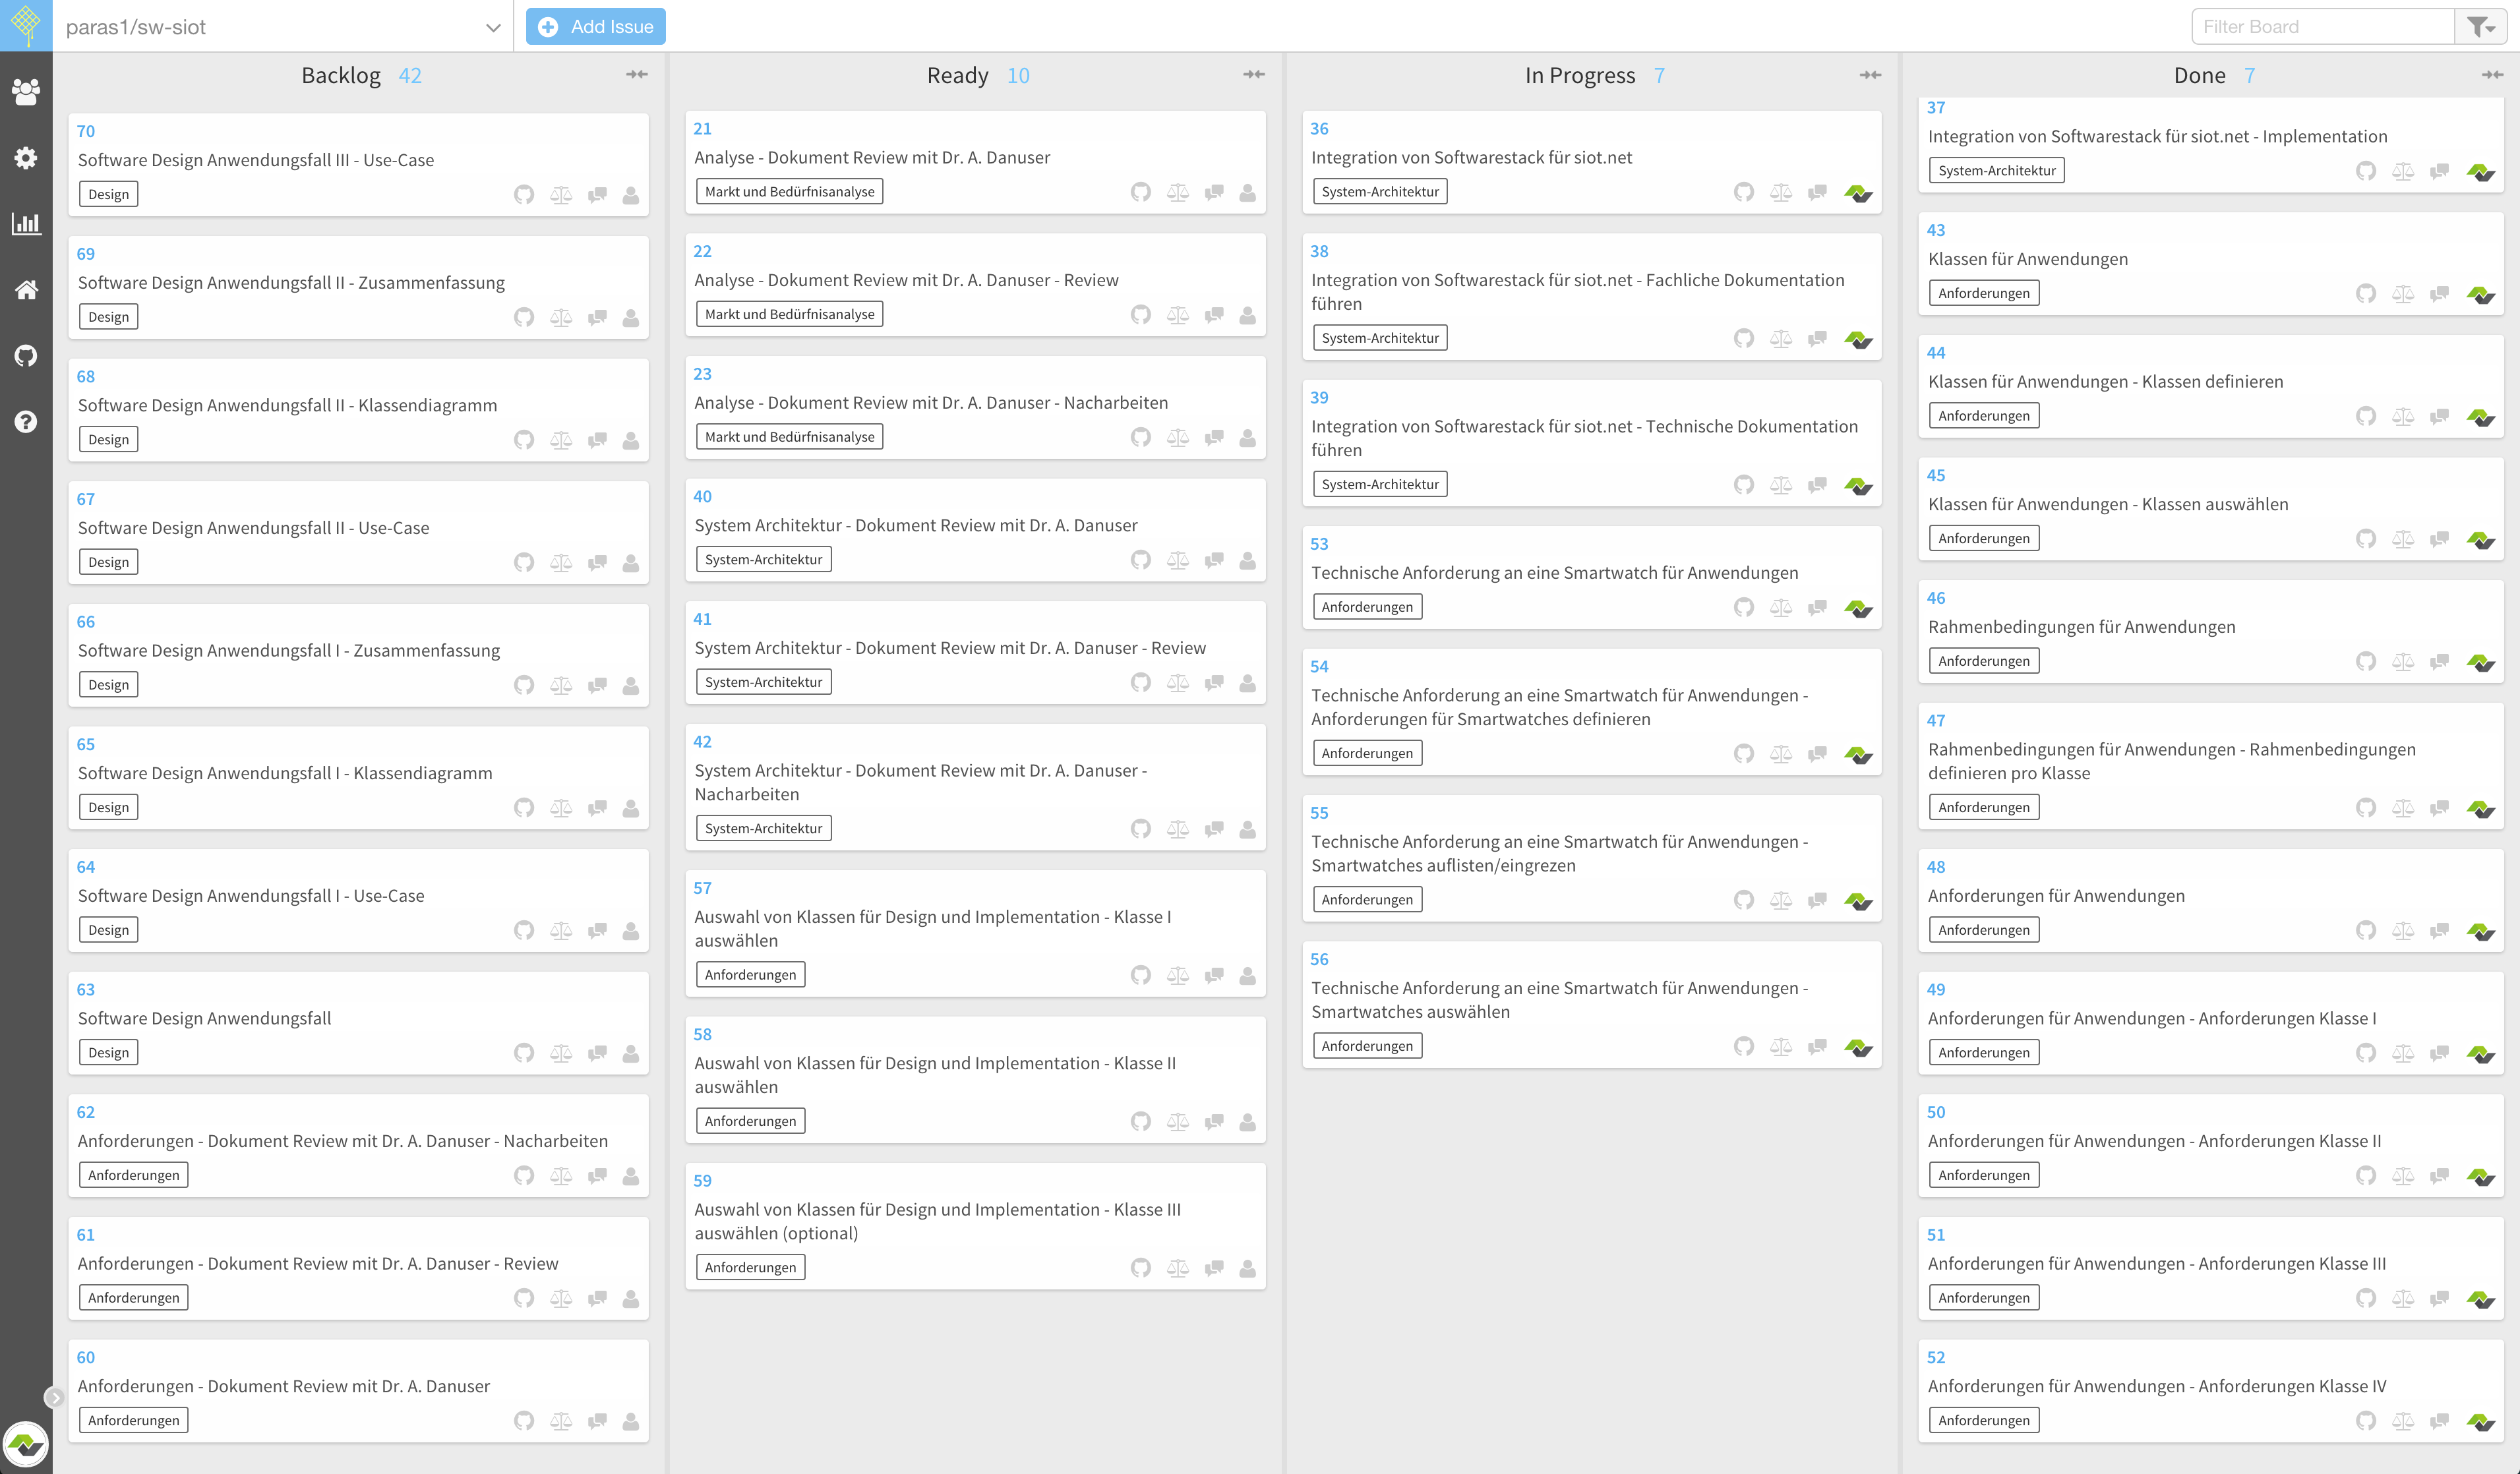
\includegraphics[scale=0.37]{98_Bilder/98_Anhang/20151210_Kanban_board}
  \caption[Kanban-Board 10.12.2015]{Kanban-Board Fortschritt am 10.12.2015}
\end{figure}
\begin{figure}[H]
  \centering
  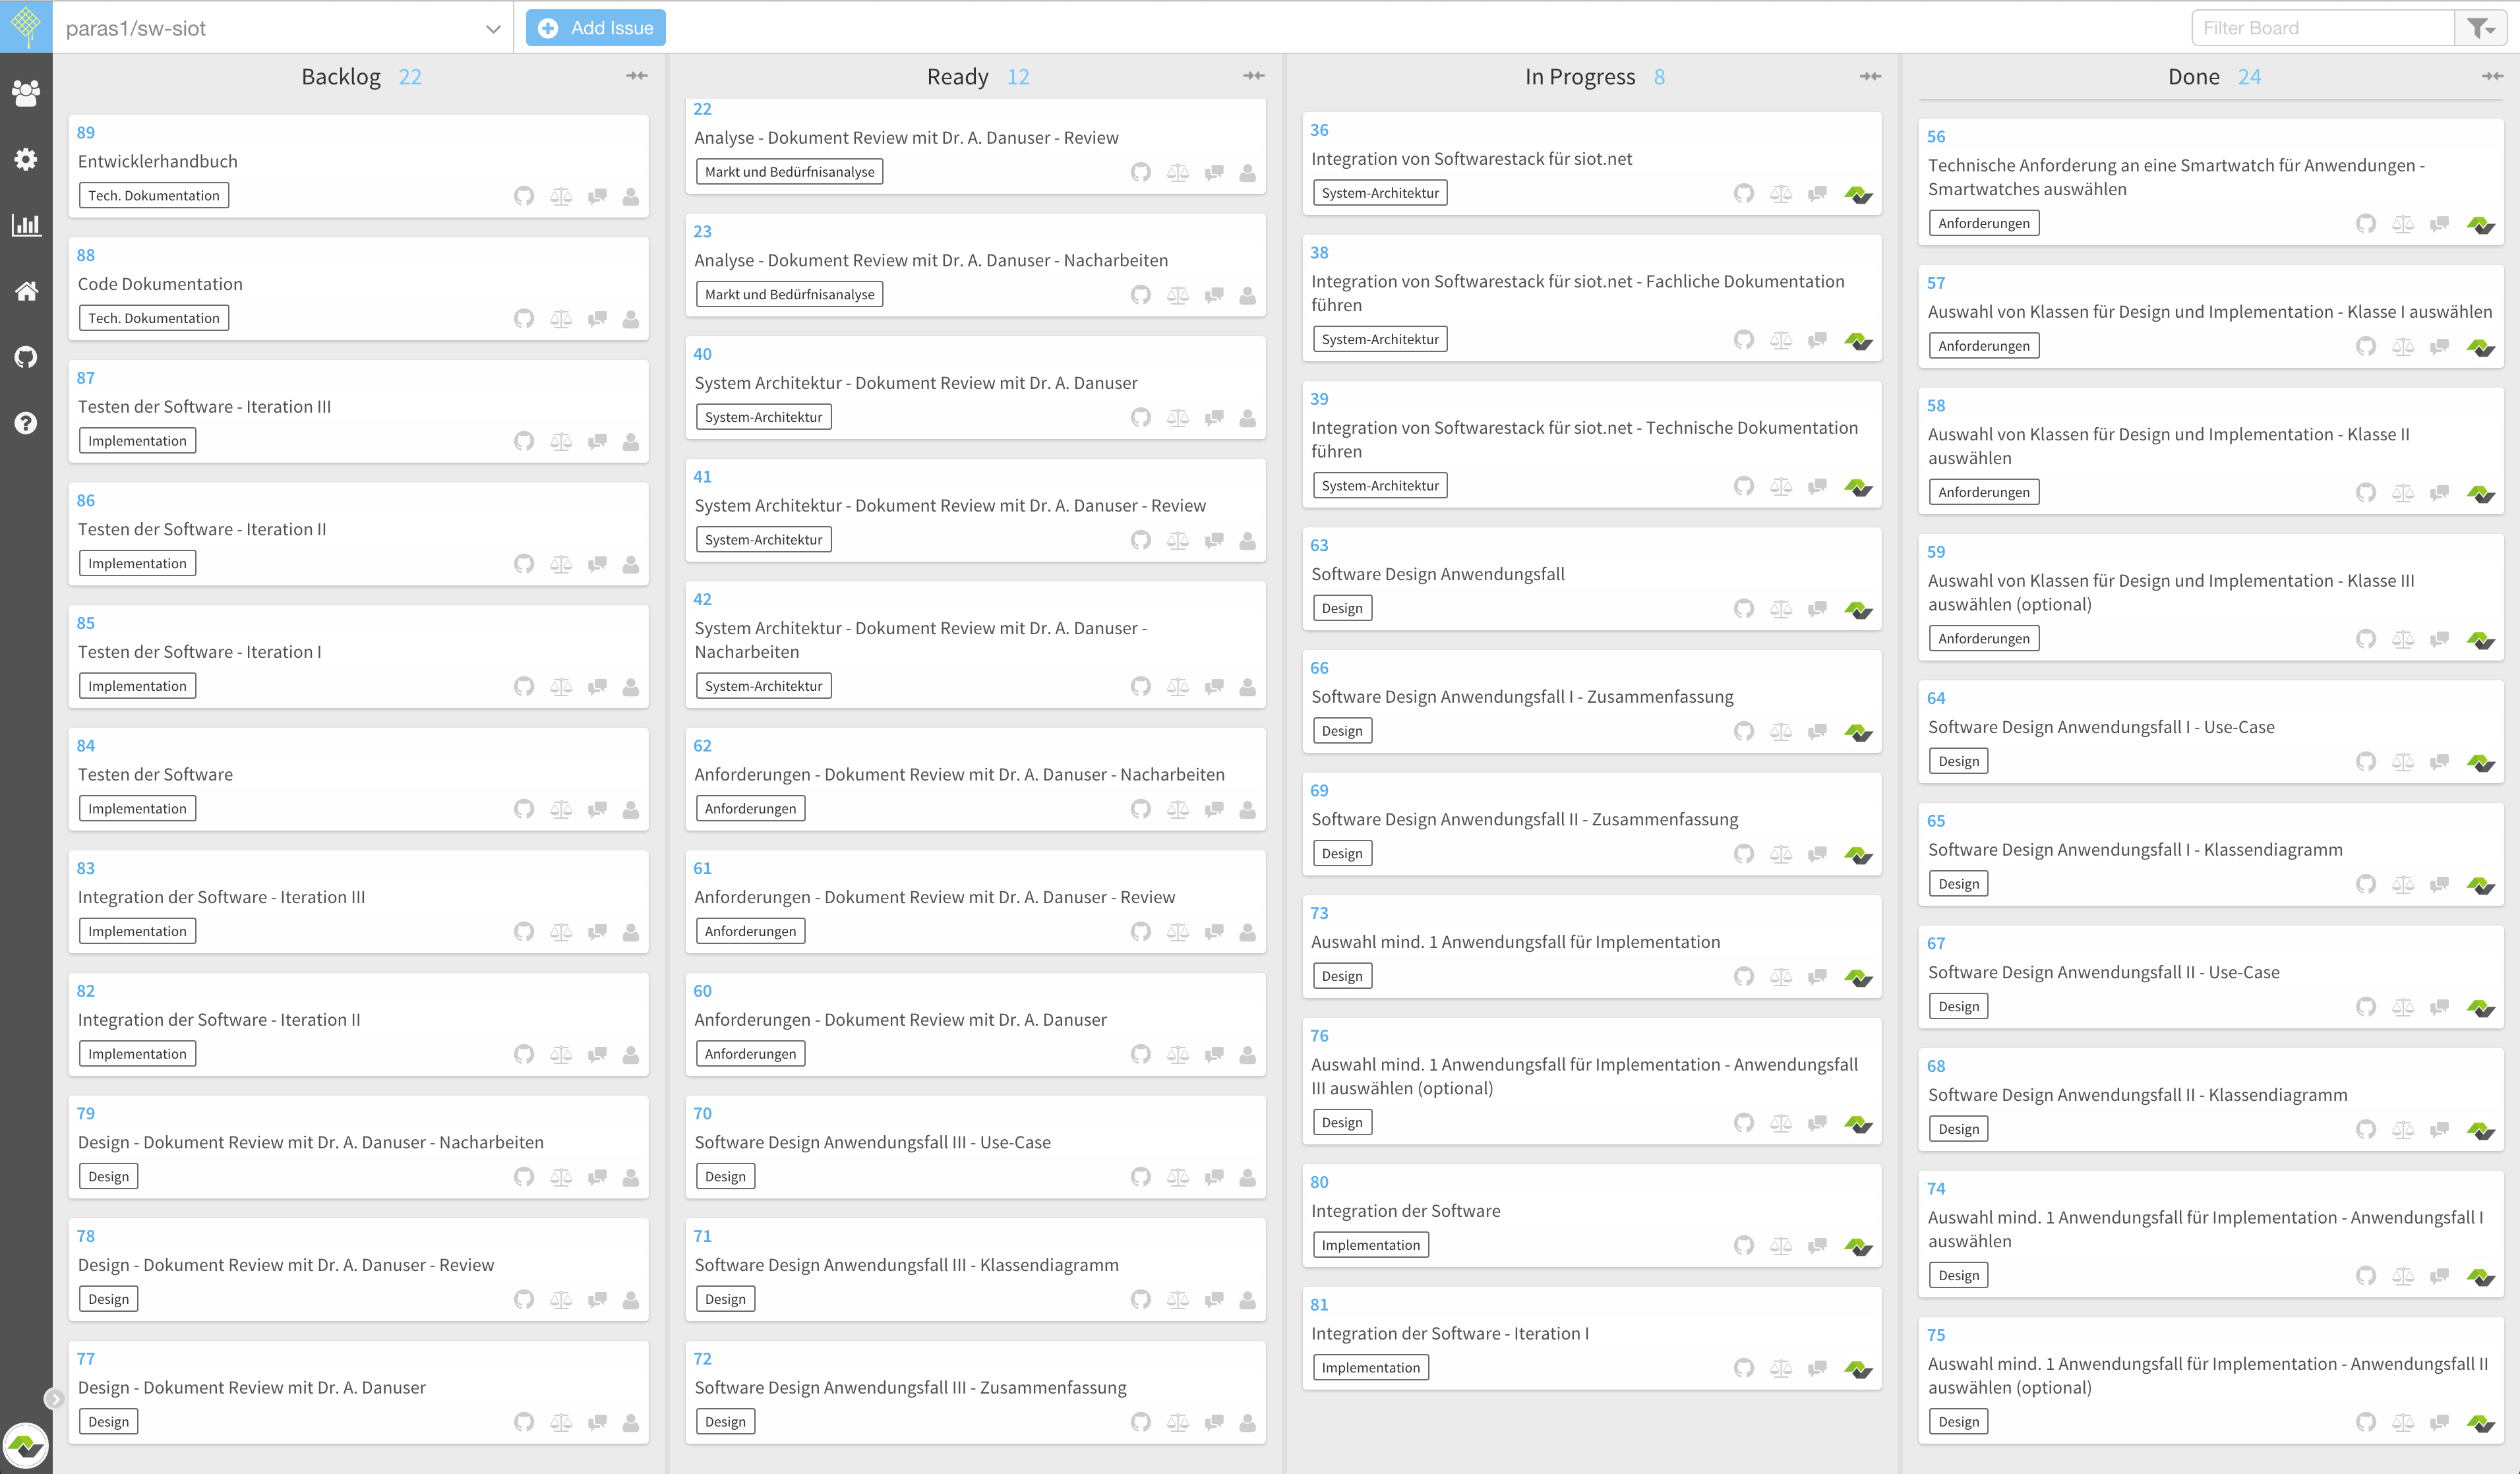
\includegraphics[scale=0.37]{98_Bilder/98_Anhang/20151216_Kanban_board}
  \caption[Kanban-Board 16.12.2015]{Kanban-Board Fortschritt am 16.12.2015}
\end{figure}
\begin{figure}[H]
  \centering
  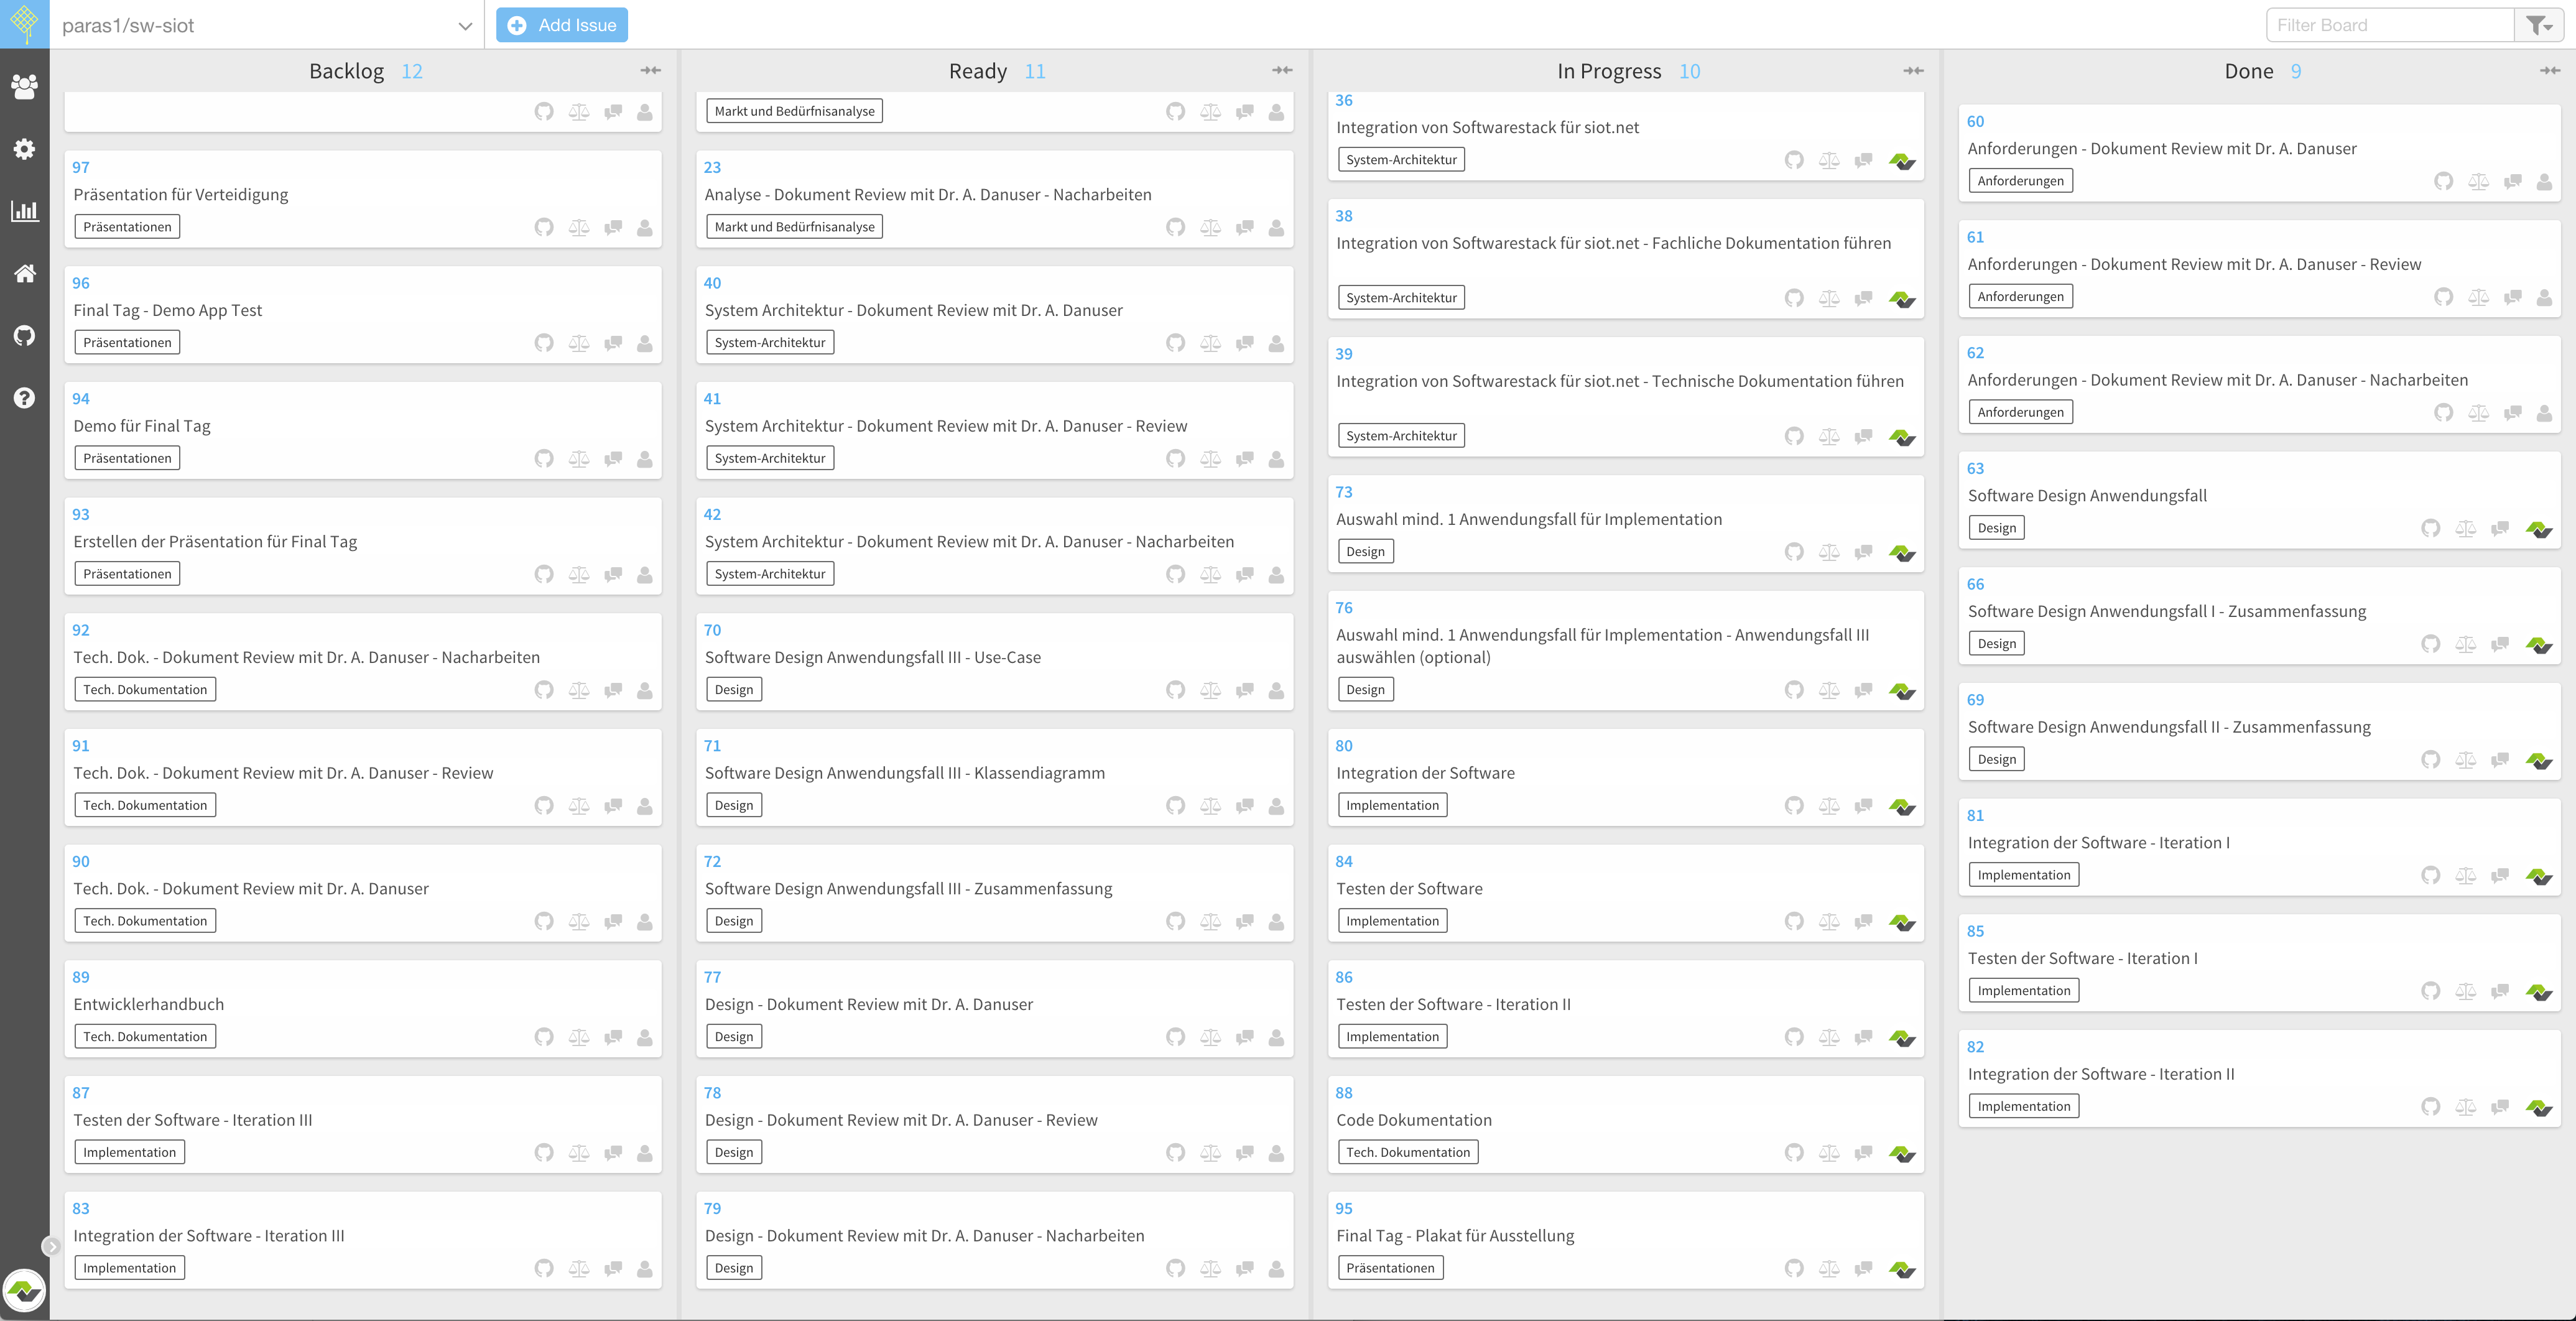
\includegraphics[scale=0.34]{98_Bilder/98_Anhang/20151223_Kanban_board}
  \caption[Kanban-Board 23.12.2015]{Kanban-Board Fortschritt am 23.12.2015}
\end{figure}
\begin{figure}[H]
  \centering
  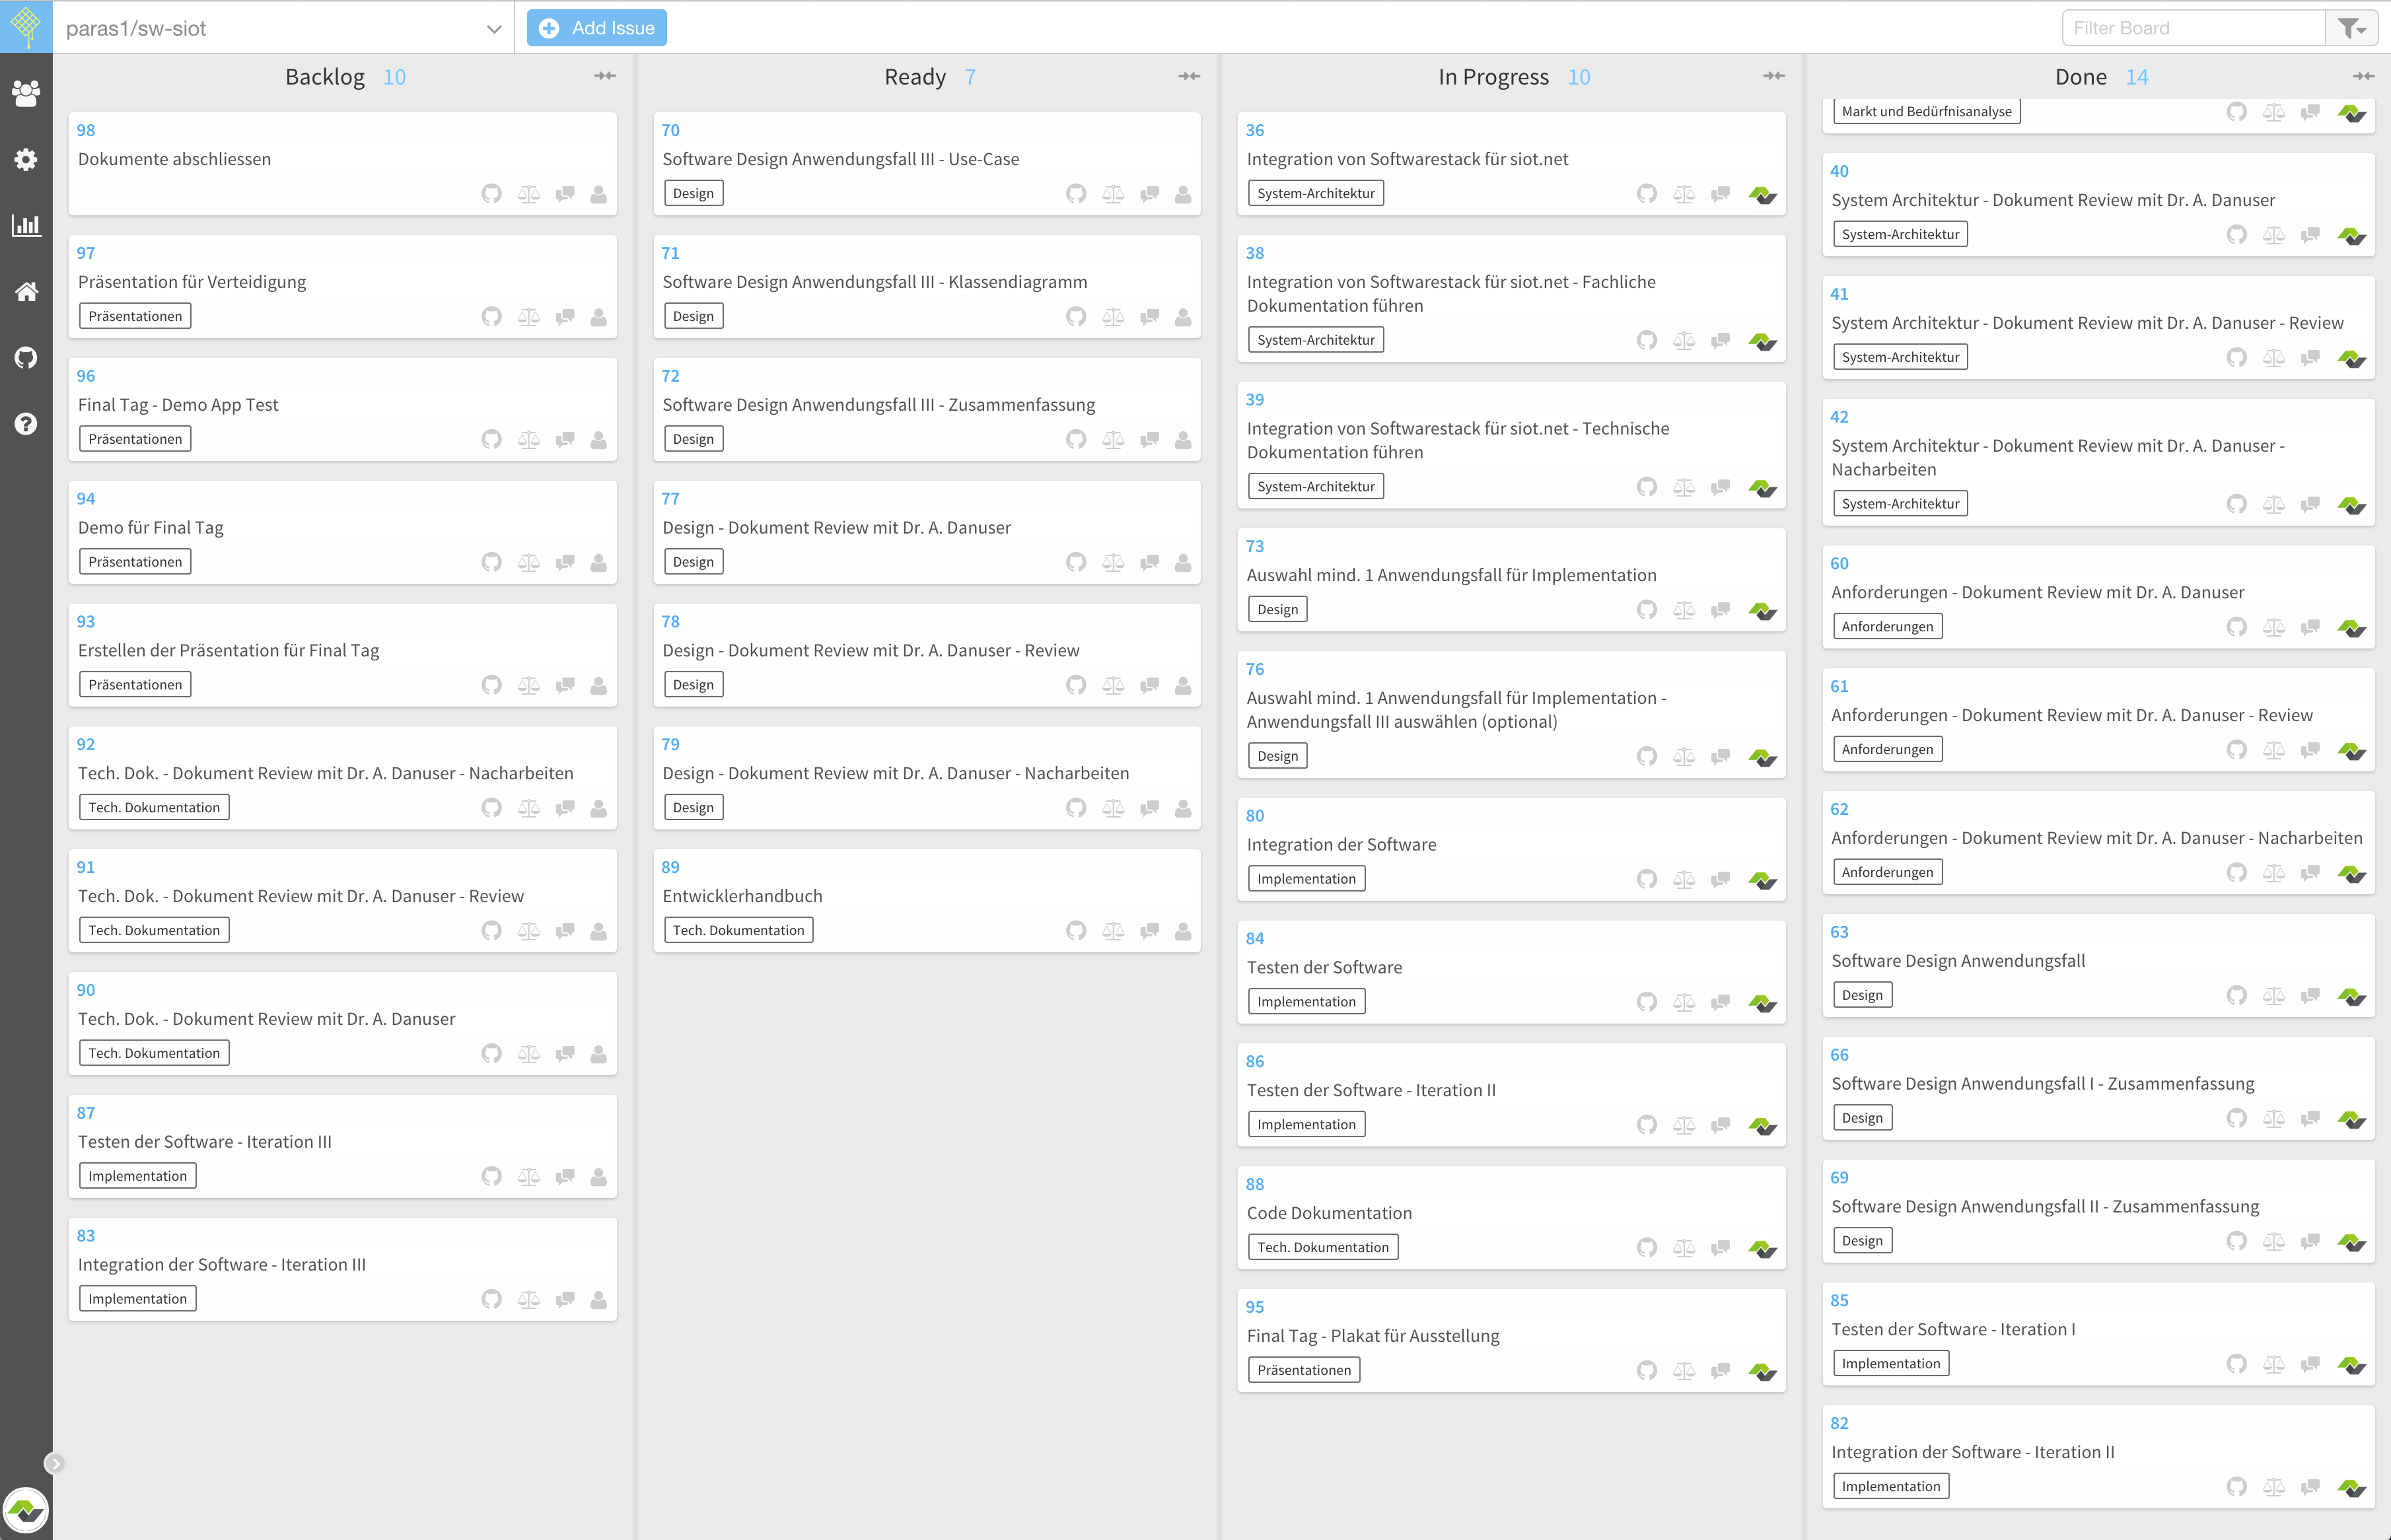
\includegraphics[scale=0.37]{98_Bilder/98_Anhang/20160102_Kanban_board}
  \caption[Kanban-Board 02.01.2016]{Kanban-Board Fortschritt am 02.01.2016}
\end{figure}
\begin{figure}[H]
  \centering
  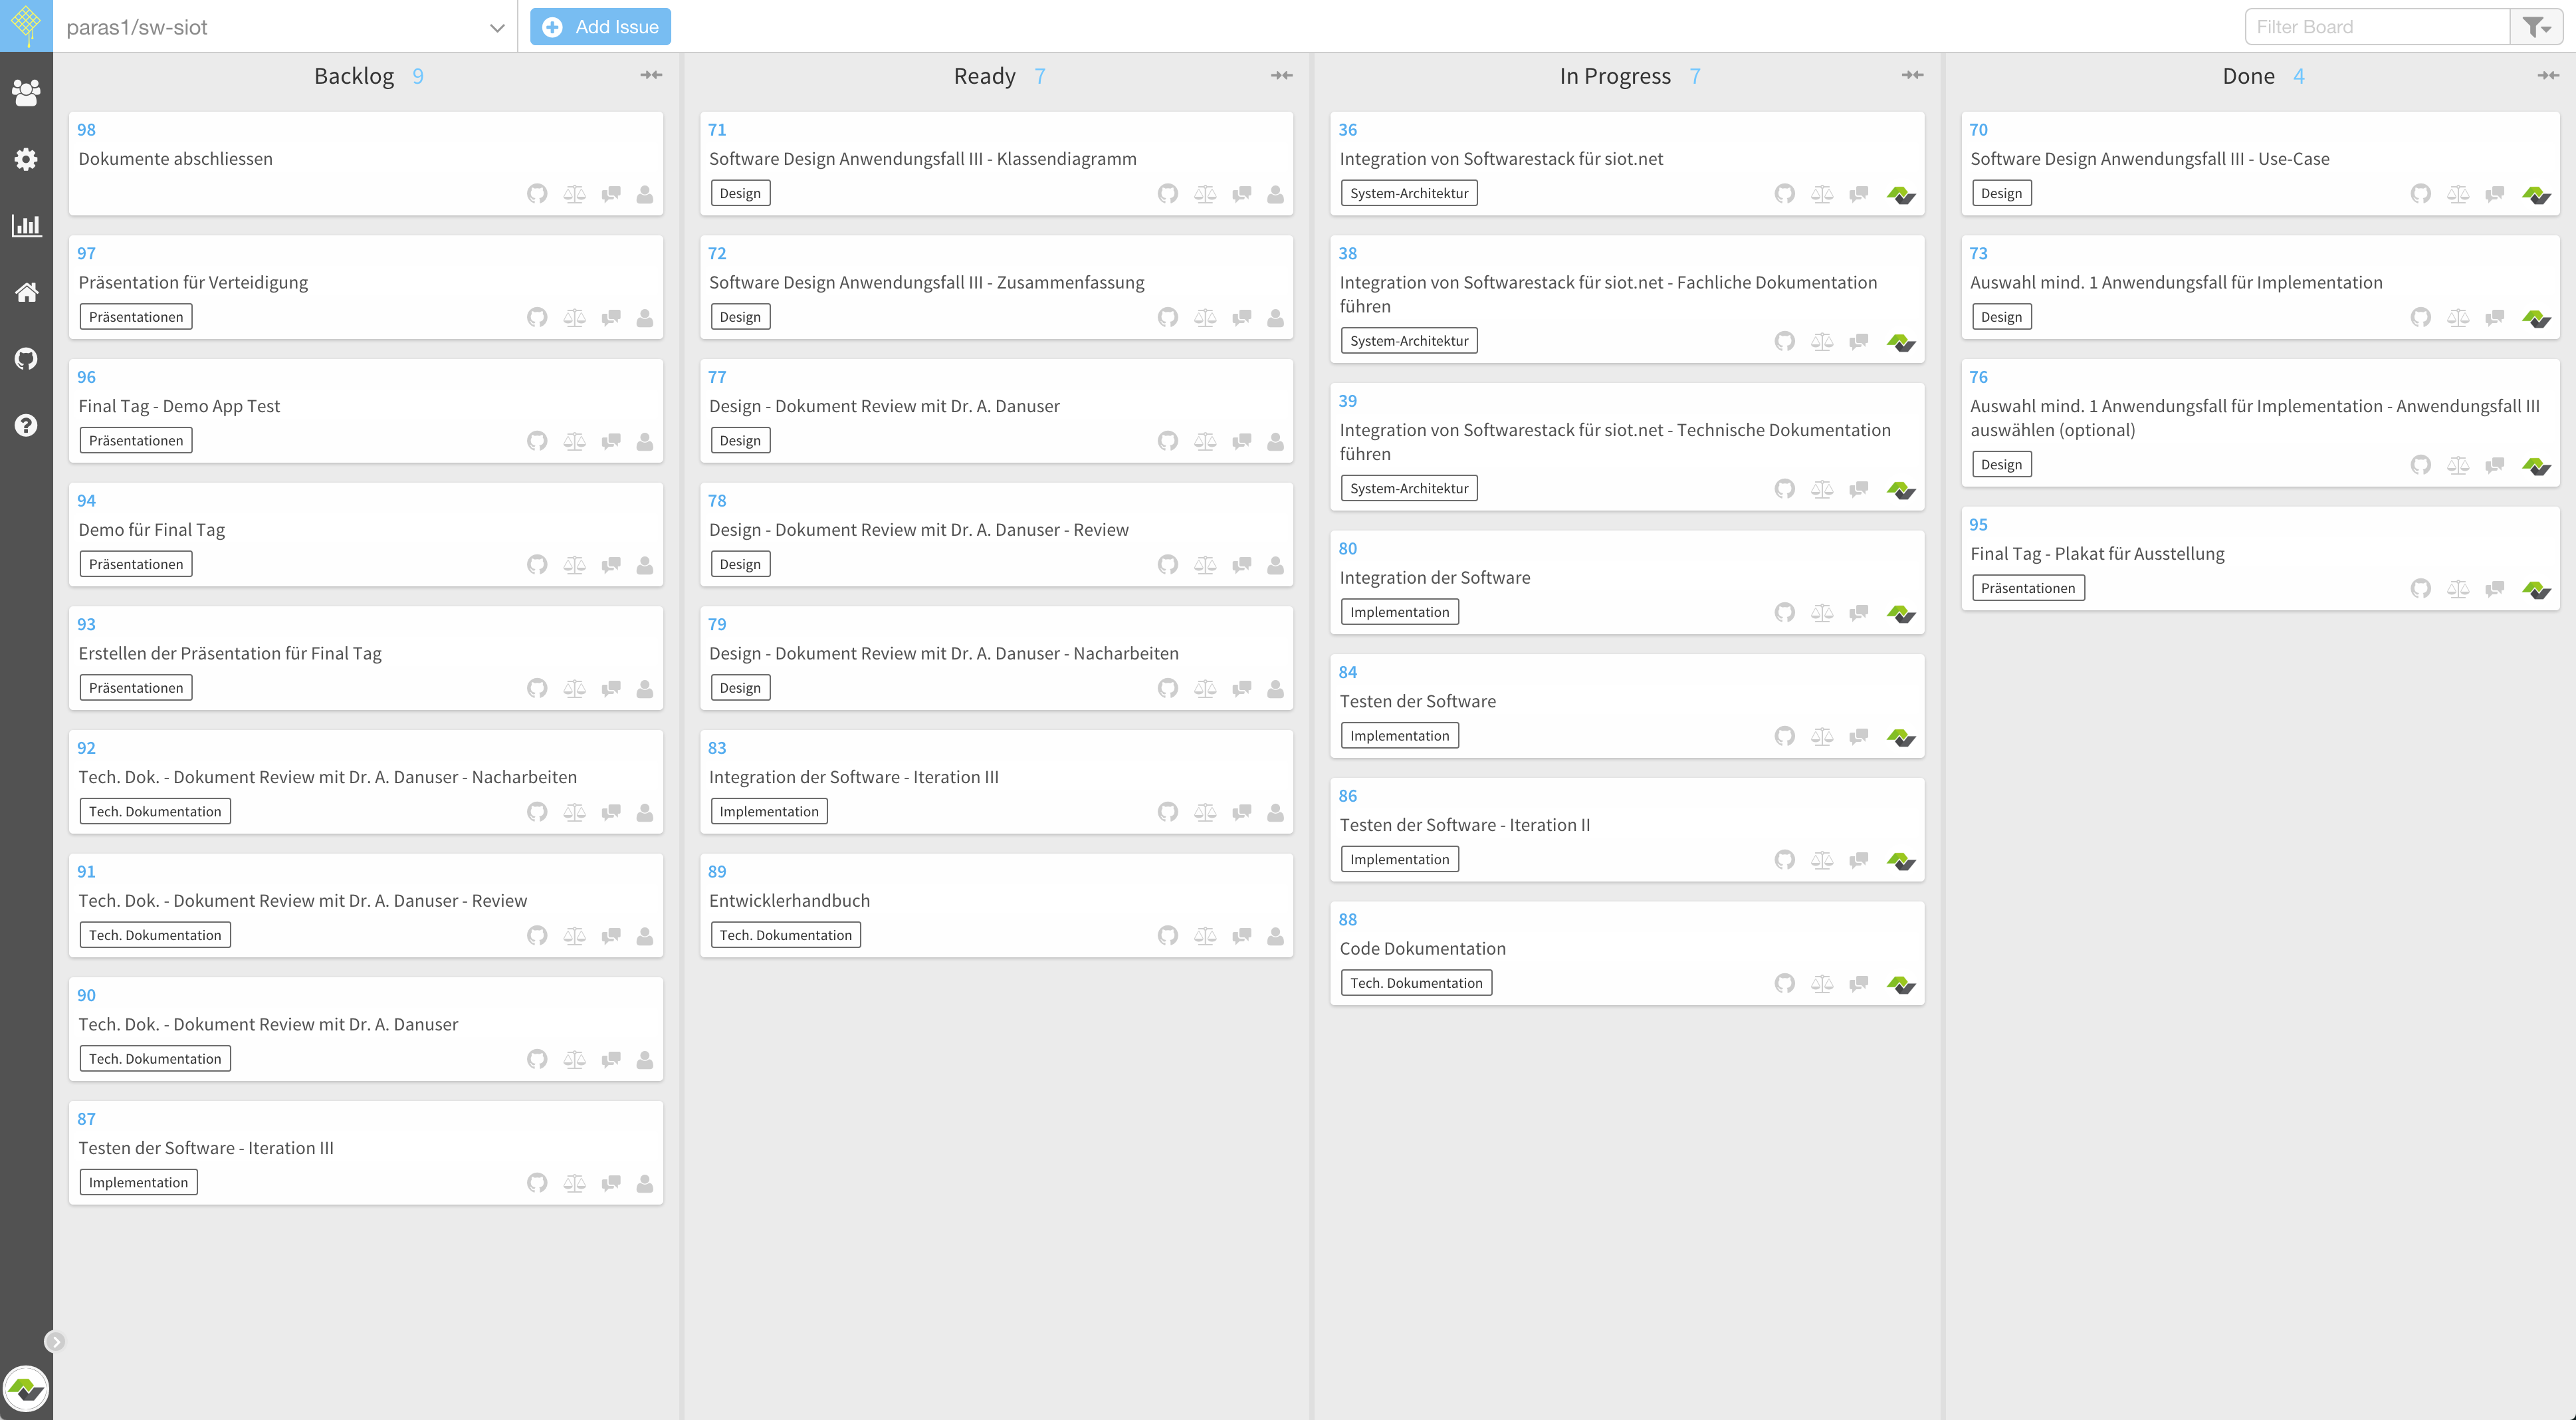
\includegraphics[scale=0.35]{98_Bilder/98_Anhang/20160105_Kanban_board}
  \caption[Kanban-Board 05.01.2016]{Kanban-Board Fortschritt am 05.01.2016}
\end{figure}
\begin{figure}[H]
  \centering
  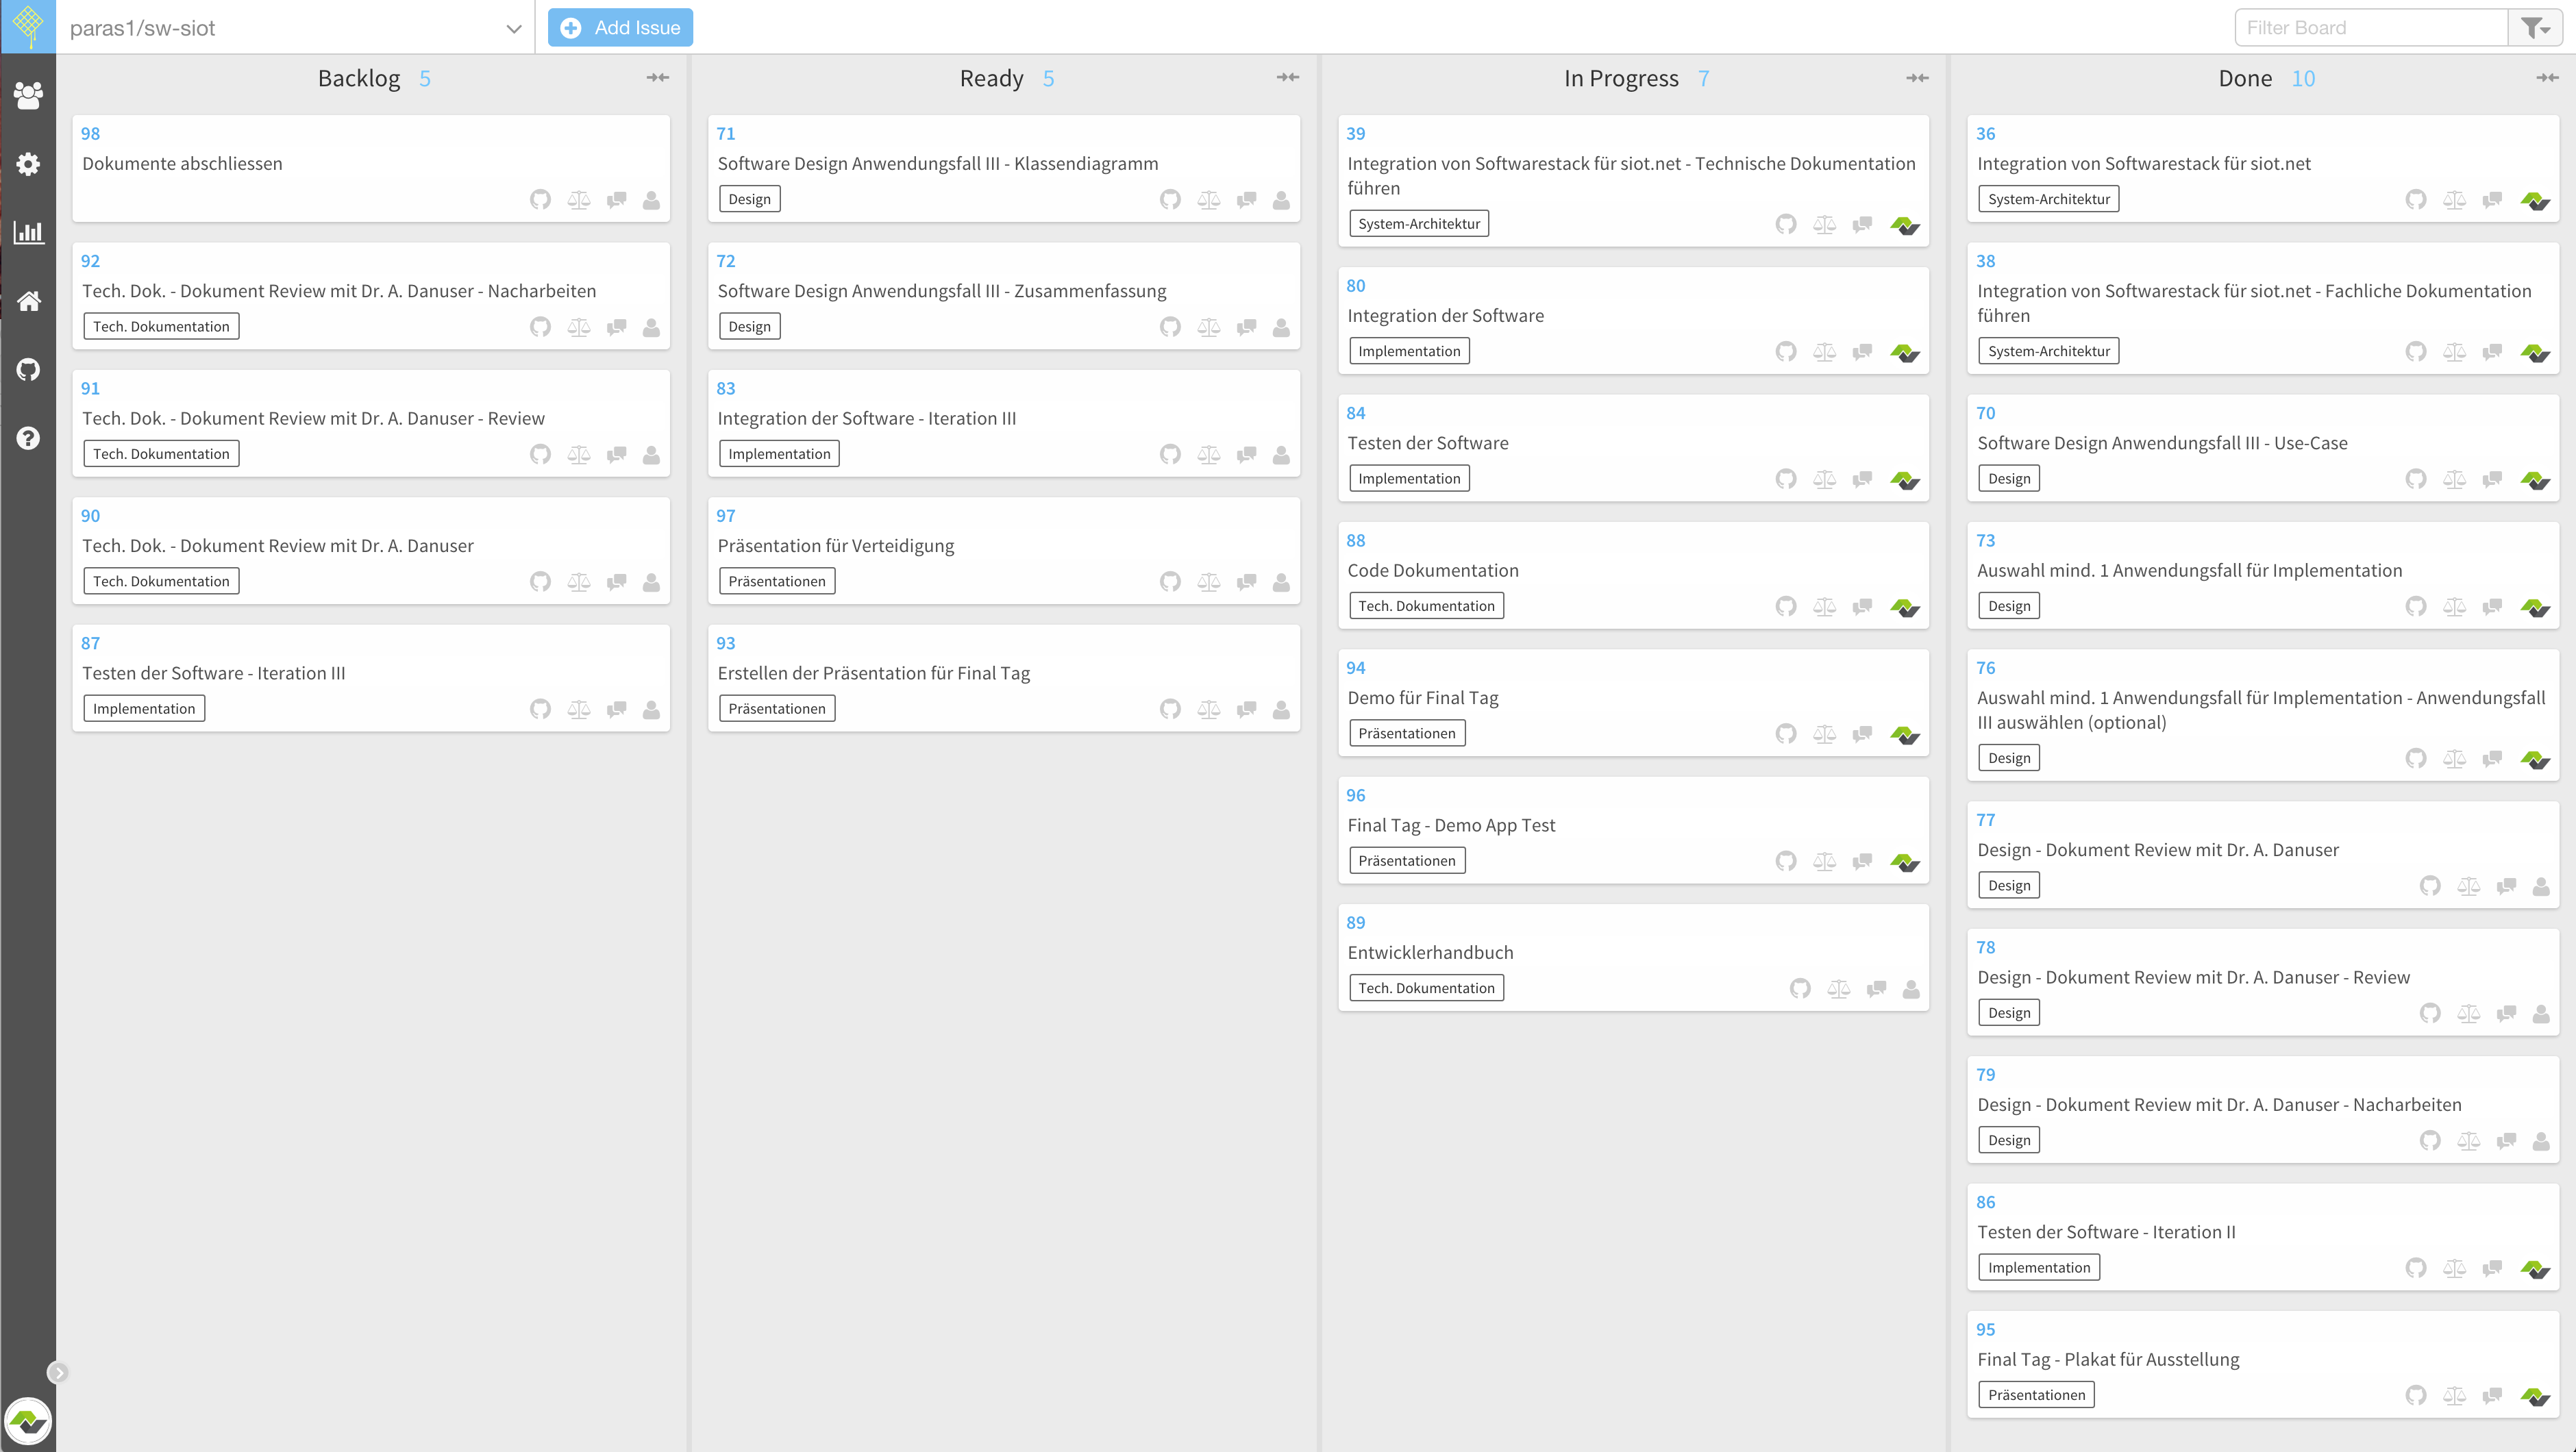
\includegraphics[scale=0.37]{98_Bilder/98_Anhang/20160110_Kanban_board}
  \caption[Kanban-Board 10.01.2016]{Kanban-Board Fortschritt am 10.01.2016}
\end{figure}
\begin{figure}[H]
  \centering
  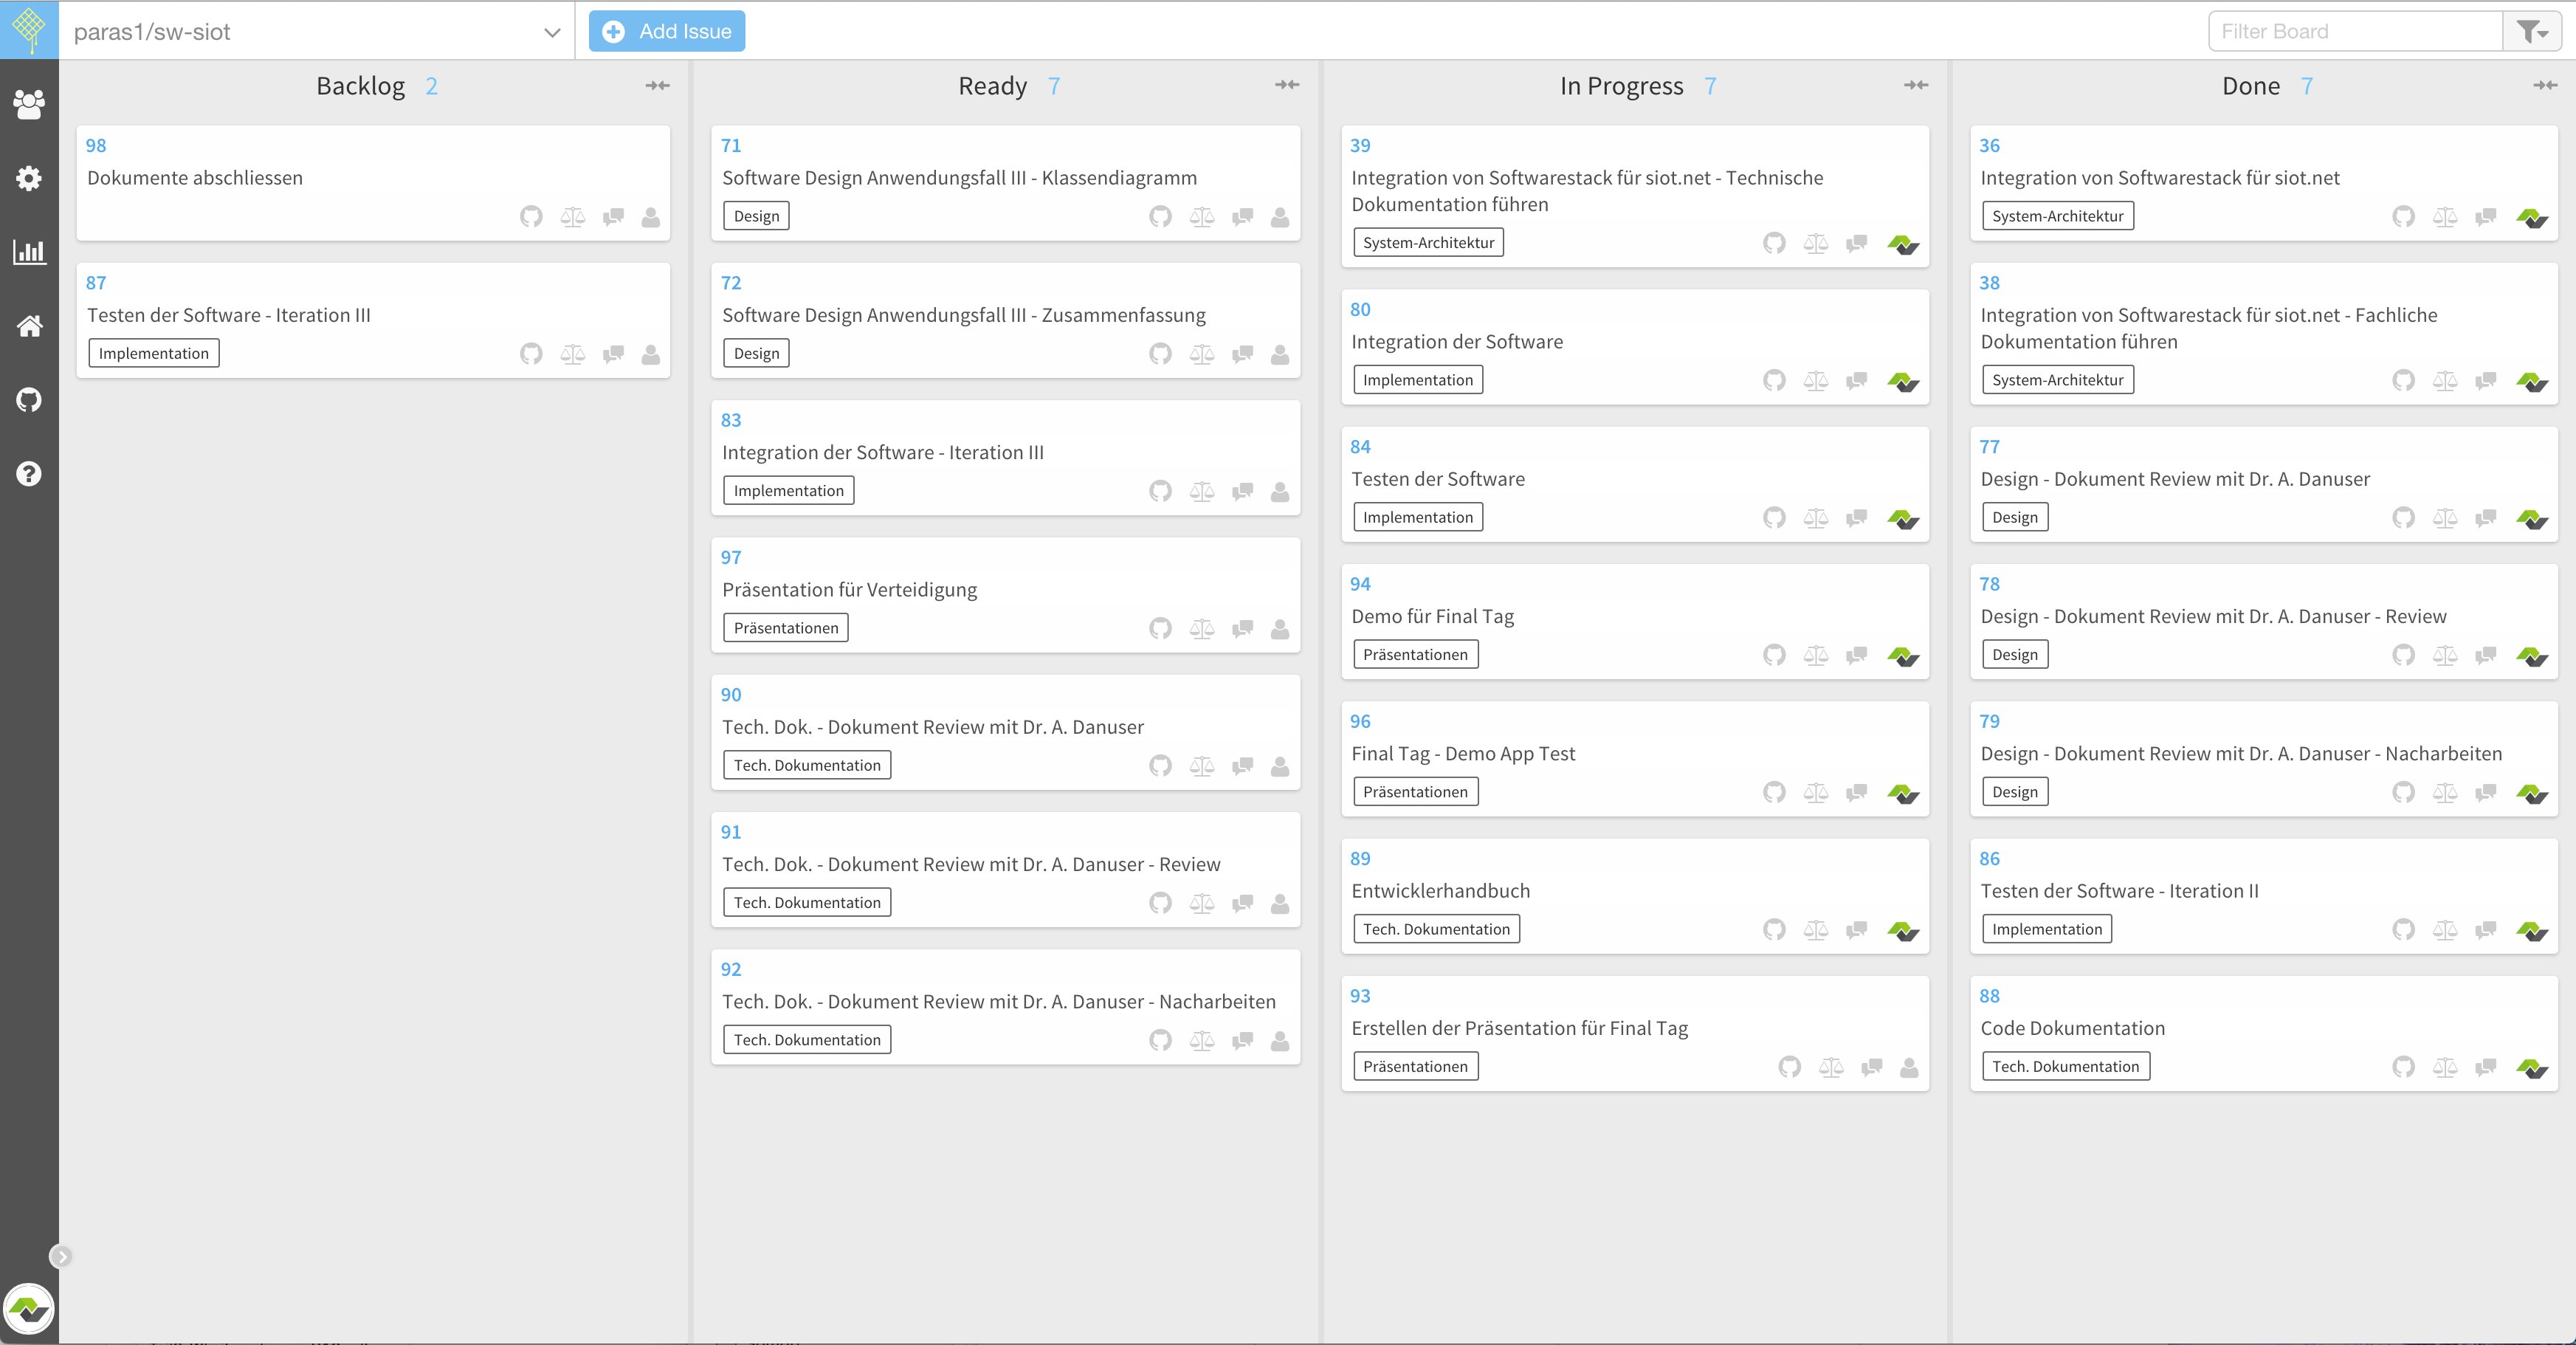
\includegraphics[scale=0.37]{98_Bilder/98_Anhang/20160114_Kanban_board}
  \caption[Kanban-Board 14.01.2016]{Kanban-Board Fortschritt am 14.01.2016}
\end{figure}
\begin{figure}[H]
  \centering
  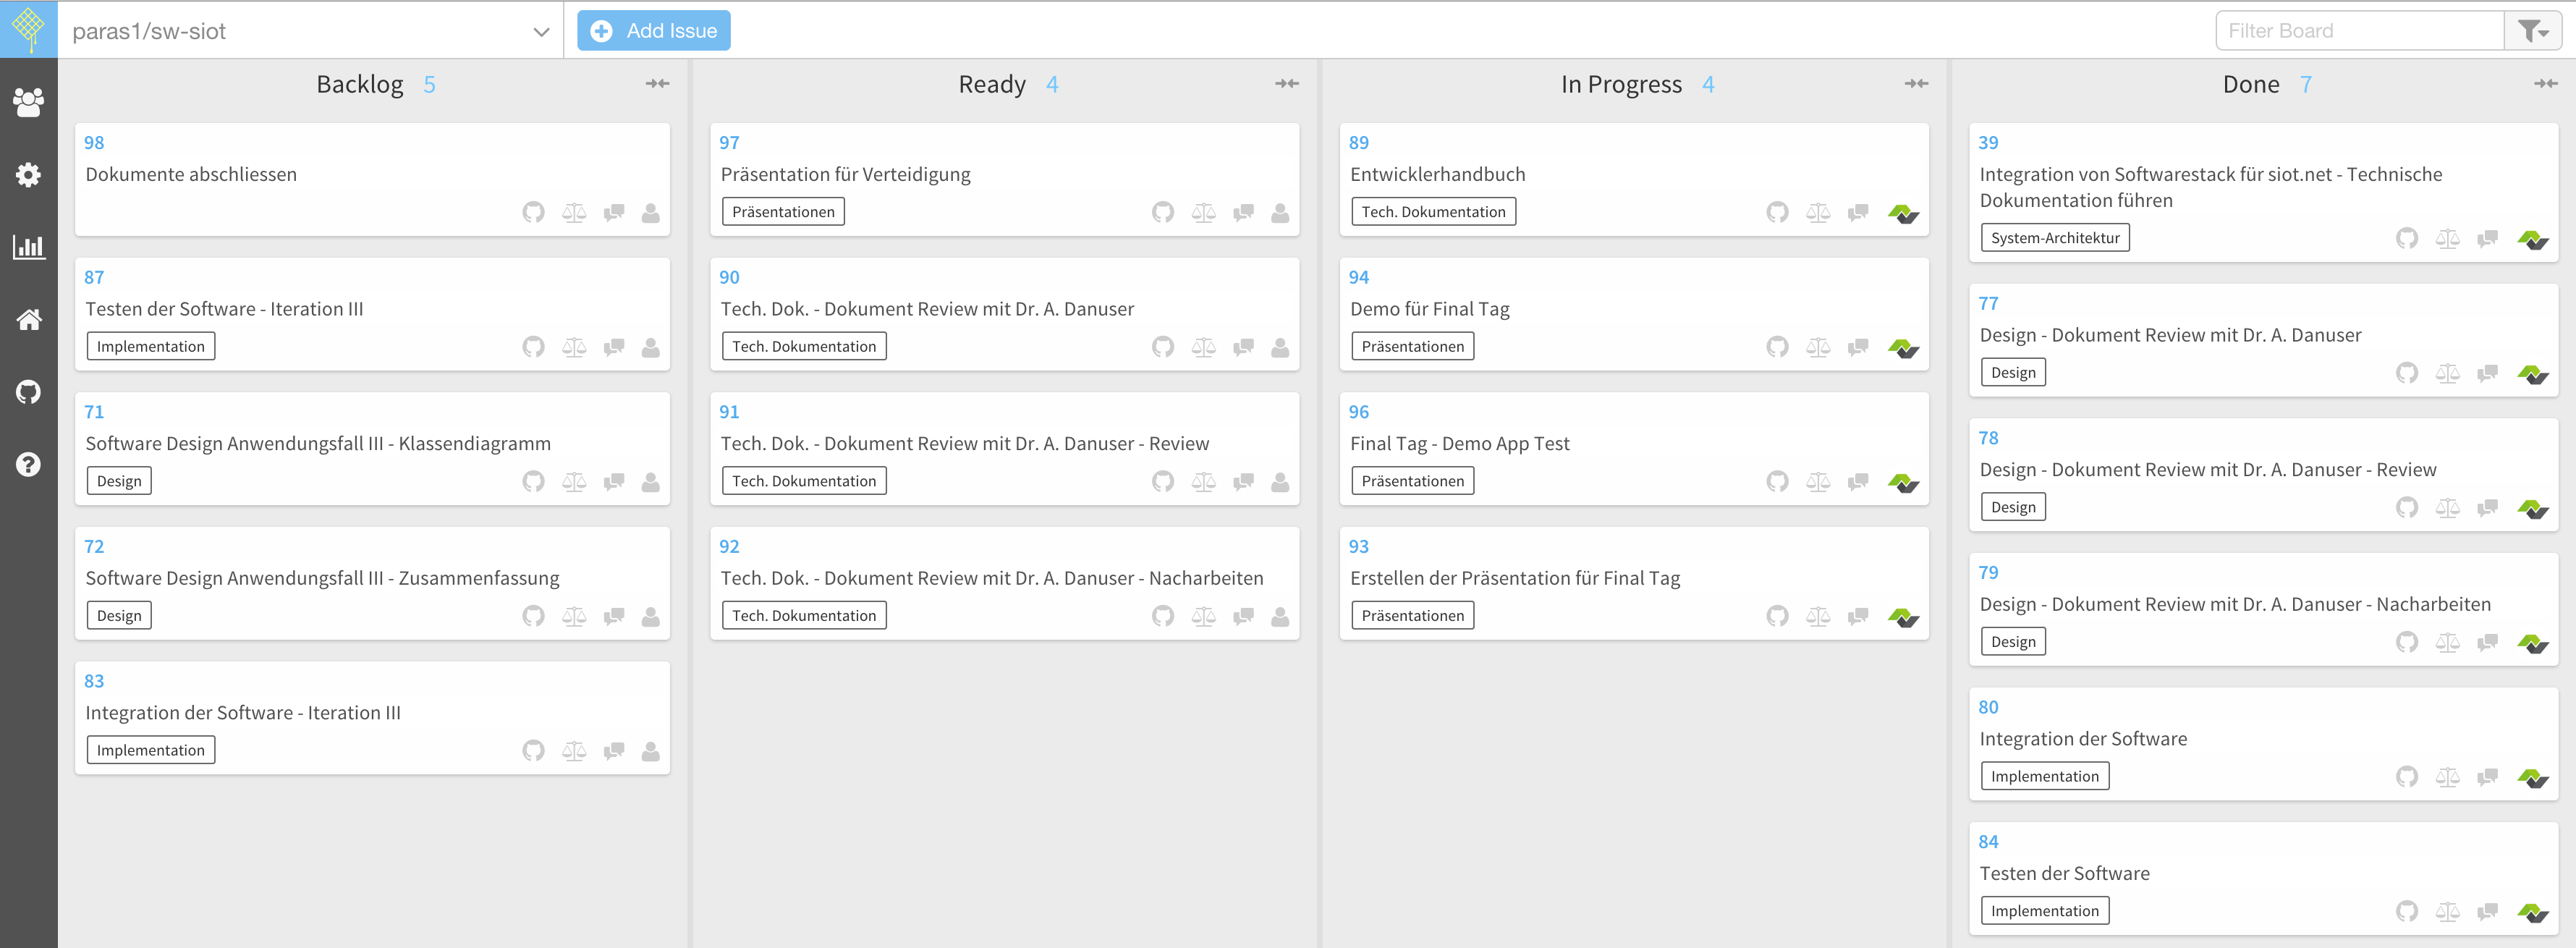
\includegraphics[scale=0.37]{98_Bilder/98_Anhang/20160117_Kanban_board}
  \caption[Kanban-Board 17.01.2016]{Kanban-Board Fortschritt am 17.01.2016}
\end{figure}
\begin{figure}[H]
  \centering
  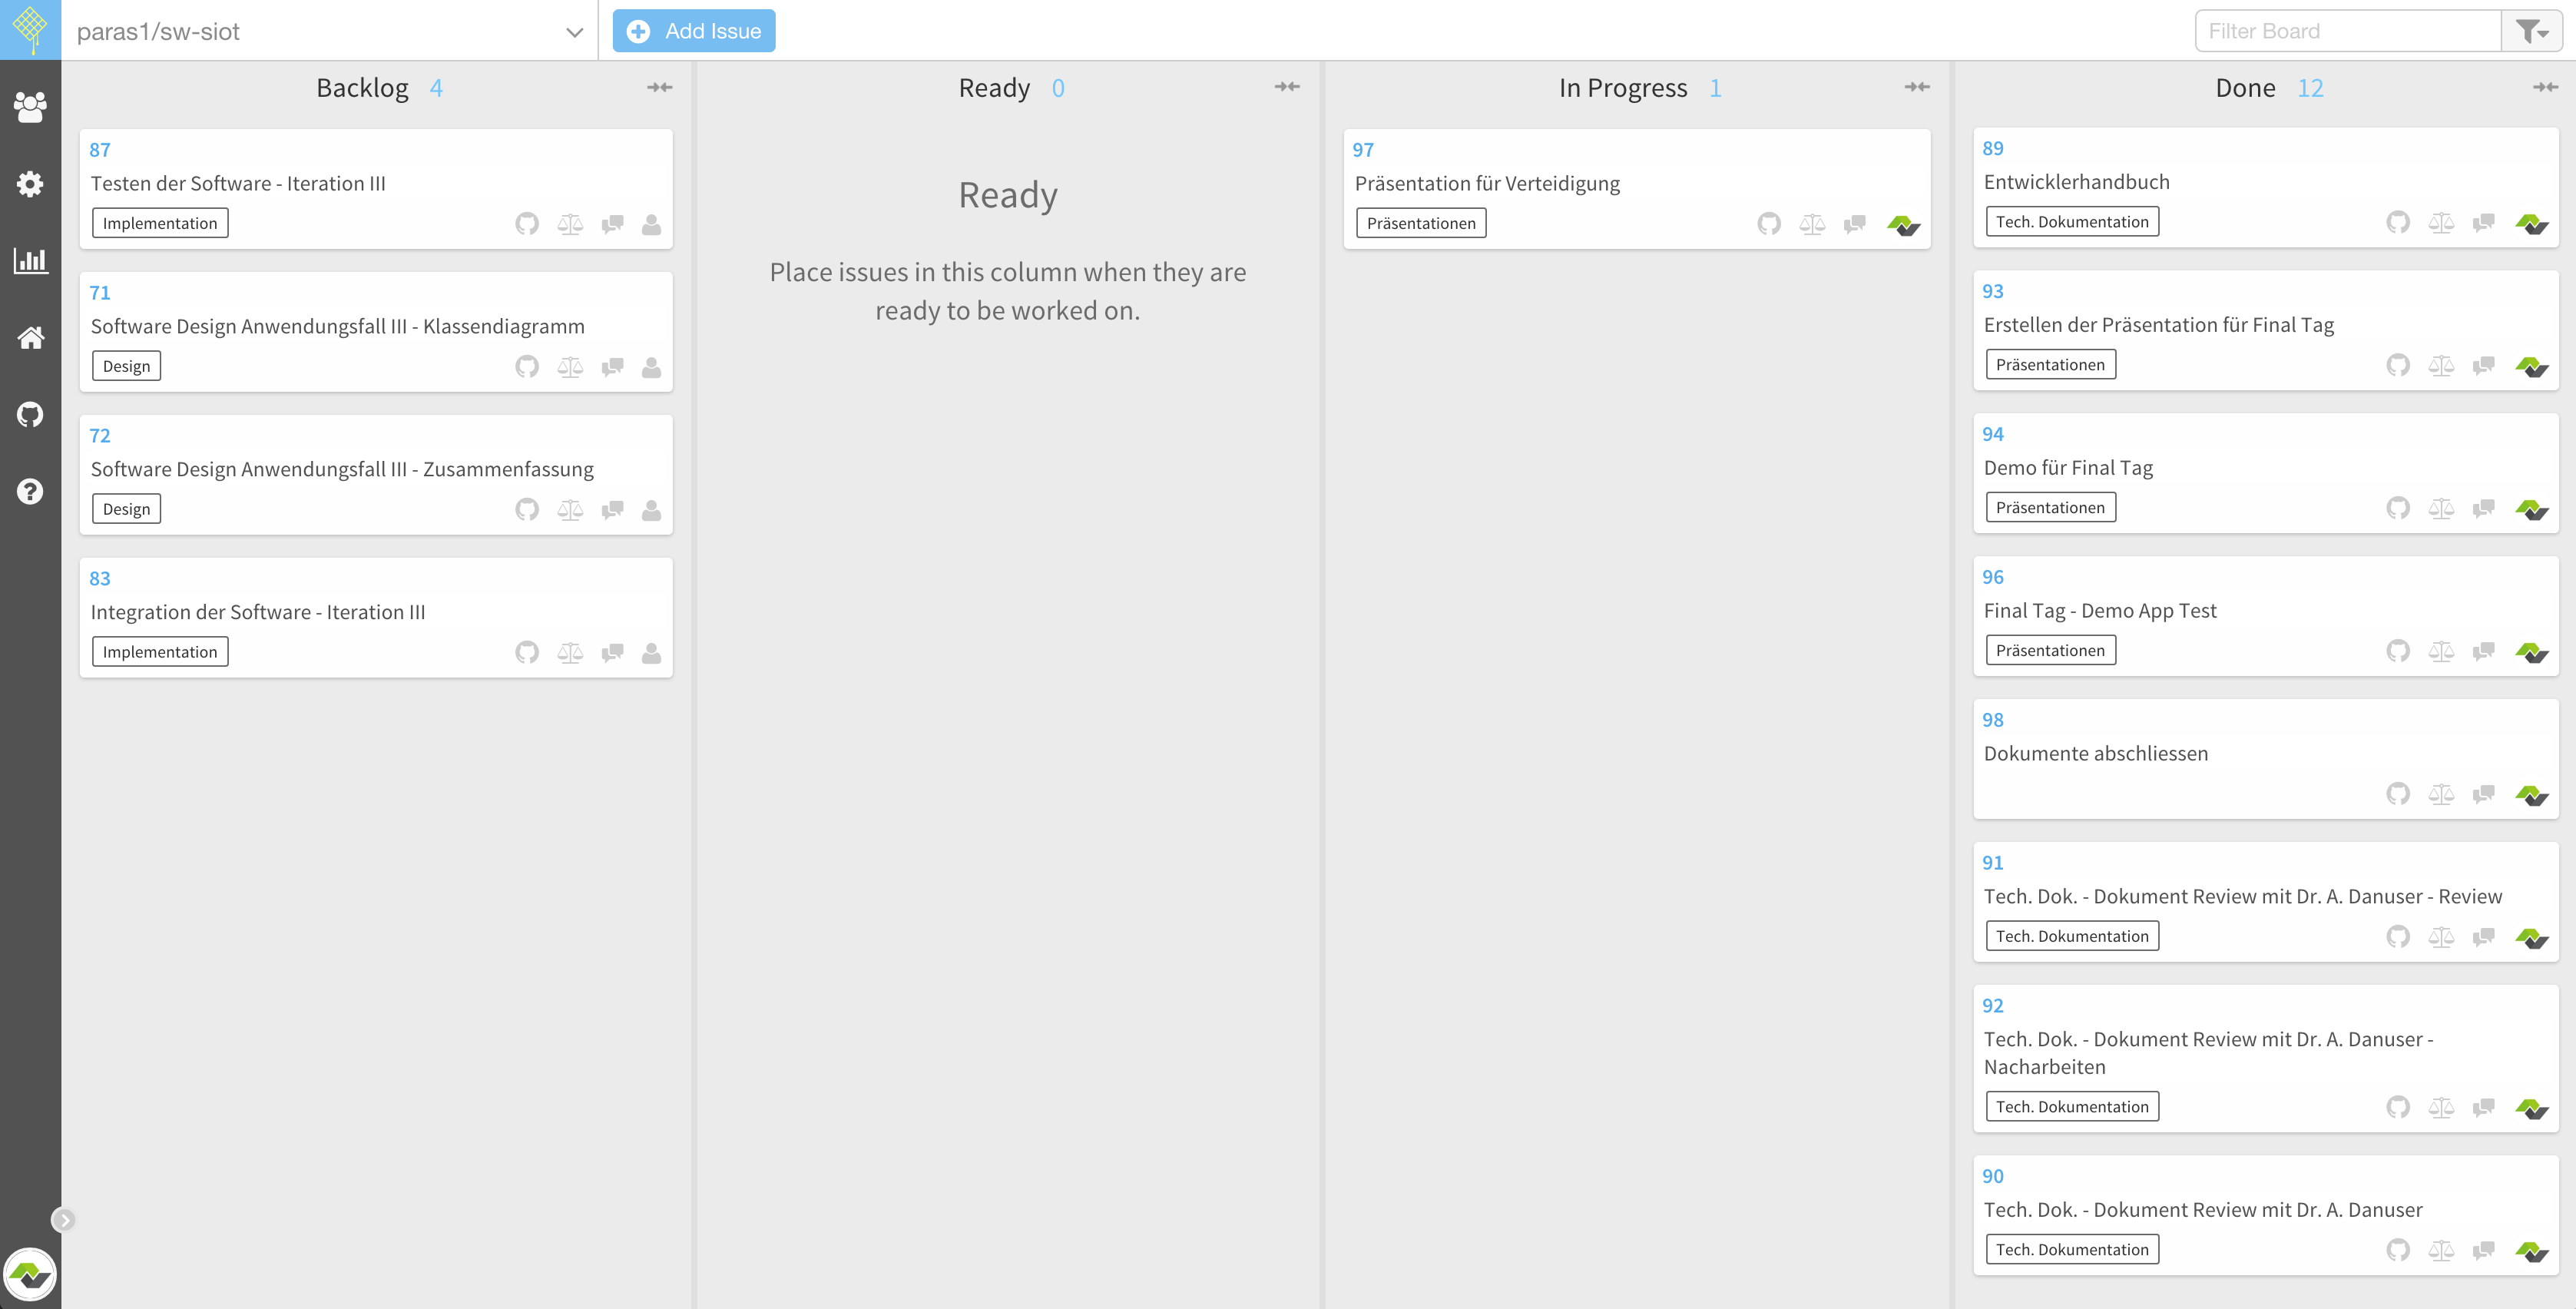
\includegraphics[scale=0.38]{98_Bilder/98_Anhang/20160121_Kanban_board}
  \caption[Kanban-Board 21.01.2016]{Kanban-Board Fortschritt am 21.01.2016}
\end{figure}
\end{landscape}
